\headline{{\textbf{\Large\sffamily TWBC Workshops:}}\\
          {\textbf{\large\sffamily A Night of Insights with David Cheshire}}}
\label{2025-11-workshop}

\topic{Potting and Tree Growth Management}
\noindent
Bonsai cultivation often begins with trees grown in nursery pots, which are typically small and lightweight. For accelerated growth, trees are commonly transplanted into progressively larger pots, such as 10–20 litre containers, allowing the tree to develop a robust root system and thicken its trunk in a relatively short period. Alternatively, trees can be planted directly in the ground for long-term growth before being repotted.  

When reducing a tree from a larger pot to a smaller one, it is crucial to gradually acclimatize the tree to its new environment. The tree will initially continue growth as if it still had access to the larger volume of soil and nutrients, so careful monitoring of watering and feeding is essential. Over time, the tree adapts to the smaller pot’s limitations, adjusting growth rates to suit the available water and nutrients. This process effectively programs the tree to understand its environment and modulate growth appropriately.  

Maintaining smaller trees rather than aiming for maximum size has practical benefits. Smaller bonsai are easier to handle, repot, and maintain, particularly as growers age. Many enthu\-siasts and nurseries have shifted focus to smaller\hfill specimens

\begin{window}[2,l,\includegraphics[width=1.0\columnwidth]{2025_11/res/workshop_cheshire.jpg},\centerline{\emph{David Cheshire sharing his natural bonsai growth methods.}}]
\end{window}
\columnbreak

\noindent
due to these practicalities, finding that smaller trees provide greater enjoyment and manageability while still achieving aesthetic goals.

\medskip
\topic{Species-Specific Insights: Sabina and Junipers}
\noindent
Certain species, such as Sabina, respond well to cutting propagation and can produce viable bonsai material in as little as three years. Sabina cuttings benefit from being kept in smaller pots, allowing for hard pruning and encouraging sprouting from older branches. Their natural low growth habit facilitates branch layering and potential natural propagation through contact with the ground.  

Junipers demonstrate notable flexibility in root and branch development. Roots can be encouraged to grow through sphagnum moss tubes wrapped in drainage mesh, creating dense and aesthetically appealing root systems over a period of less than a year. Exposing these roots gradually adds character and visual interest, transforming young, simple cuttings into complex, mature-looking trees. Branches of junipers can be trained using a combination of wiring and natural growth patterns. Flexible shoots allow semi-cascade forms to develop organically, with branches growing back towards light and creating natural movement without rigid wiring. This approach mimics traditional Japanese bonsai techniques where trees are allowed to find their natural shape over time.

\medskip
\topic{Shaping and Wiring Techniques}
\noindent
Bonsai shaping is not solely dependent on wiring every branch. Strategic use of existing wires within the root system or pot can adjust branch positions over time, reducing labor-intensive wiring while guiding growth effectively. Young trees are often wired minimally to support structure or encourage desired growth direction, while older branches may be pruned or cut to buds that naturally grow in preferred directions.  

Observation and patience are critical in shaping. Trees respond to light, gravity, and environmental conditions, allowing adjustments over seasons. Natural movement can be emphasized by tilting, repotting, or adjusting branch angles to create twists and semi-cascade effects. This approach reduces reliance on intensive wiring and prioritizes a more organic development process, reflecting the nuanced techniques used in Japanese bonsai cultivation.

\medskip
\topic{Species Selection and Native Trees}
\noindent
Native species such as blackthorn and marvellous plums (Marabella) offer unique advantages for bonsai enthusiasts. These species produce early flowers, creating striking seasonal interest. However, they present challenges, including limited fibrous root systems, which complicates collection and propagation. Preparation and careful extraction are critical to minimize tree loss.  

Exposing roots and positioning the tree to encourage natural twists and growth patterns can enhance character. By repotting and adjusting growth angles over successive seasons, even relatively young trees develop intricate structures resembling older specimens. Slow growth, combined with selective pruning and environmental adaptation, is key to achieving naturalistic, visually compelling bonsai.

\end{multicols}

\begin{center}
\begin{minipage}[b]{.45\textwidth}
\includegraphics[angle=0,origin=c,width=1.0\textwidth]{2025_11/res/workshop_sebina_01.jpg}
\end{minipage}\quad
\begin{minipage}[b]{.45\textwidth}
\includegraphics[angle=0,origin=c,width=1.0\textwidth]{2025_11/res/workshop_sebina_03.jpg}
\end{minipage}
\medskip

\begin{minipage}[b]{.45\textwidth}
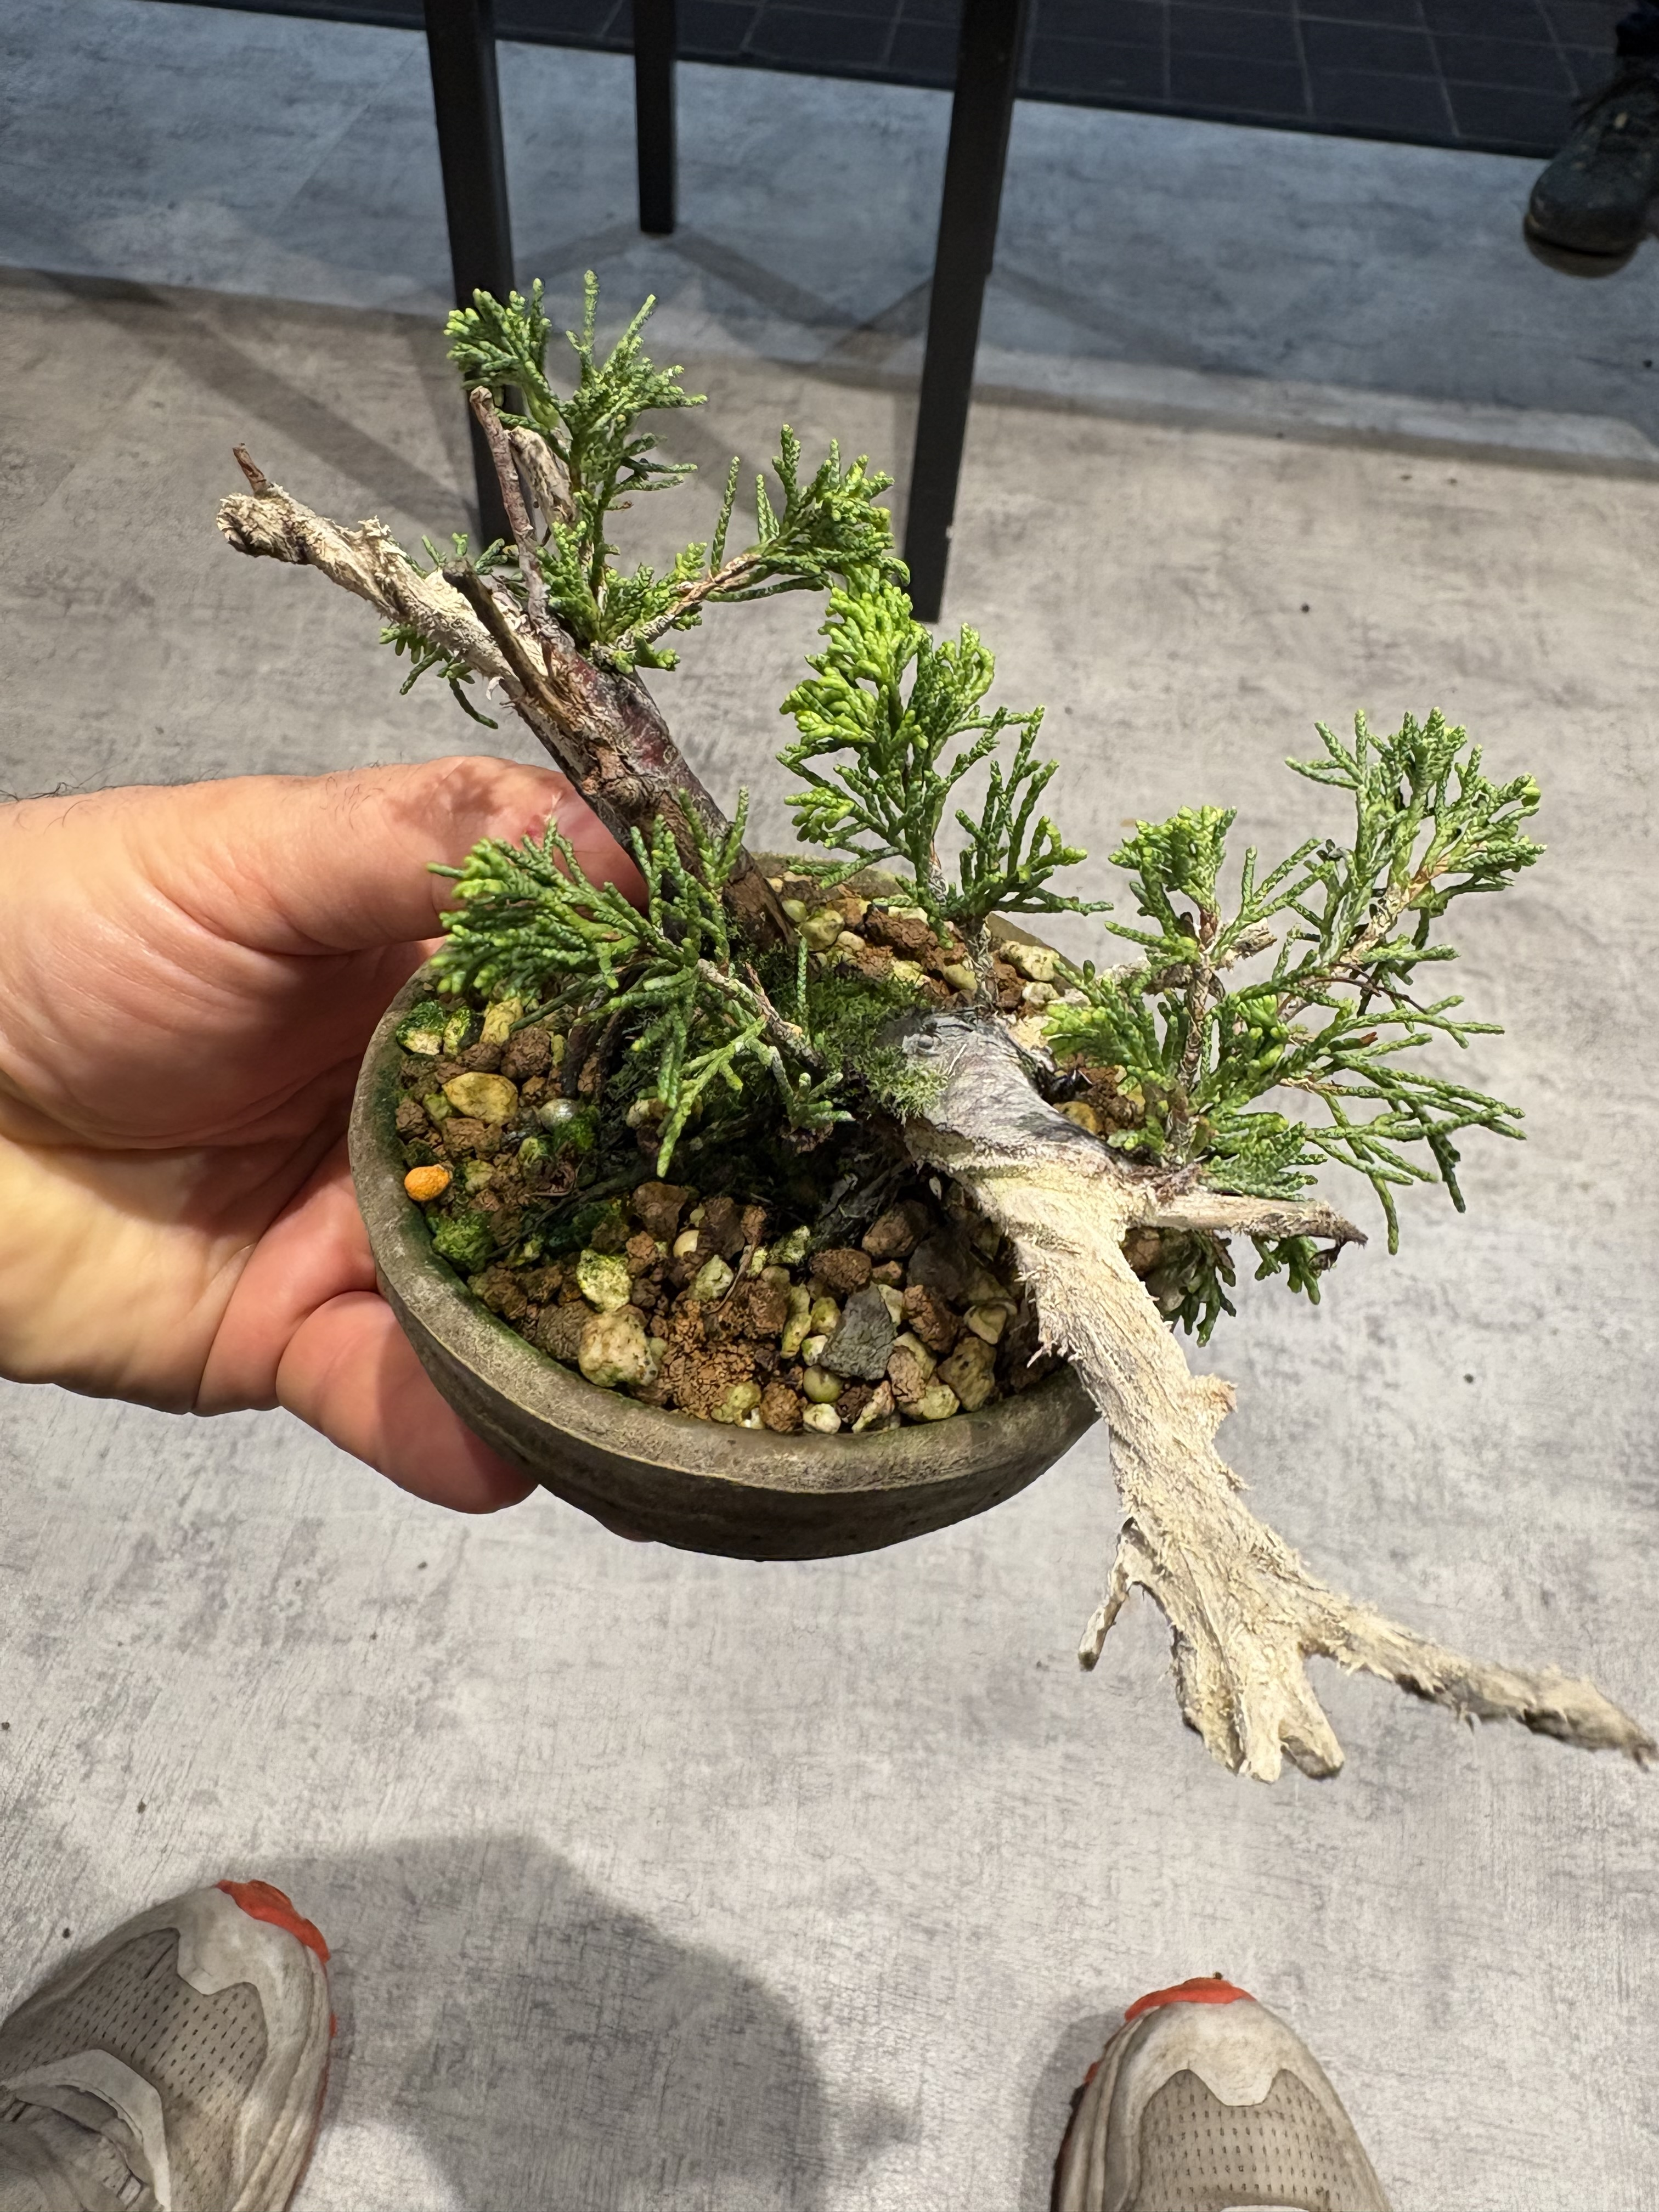
\includegraphics[angle=0,origin=c,width=1.0\textwidth]{2025_11/res/workshop_sebina_02.jpg}
\end{minipage}\quad
\begin{minipage}[b]{.45\textwidth}
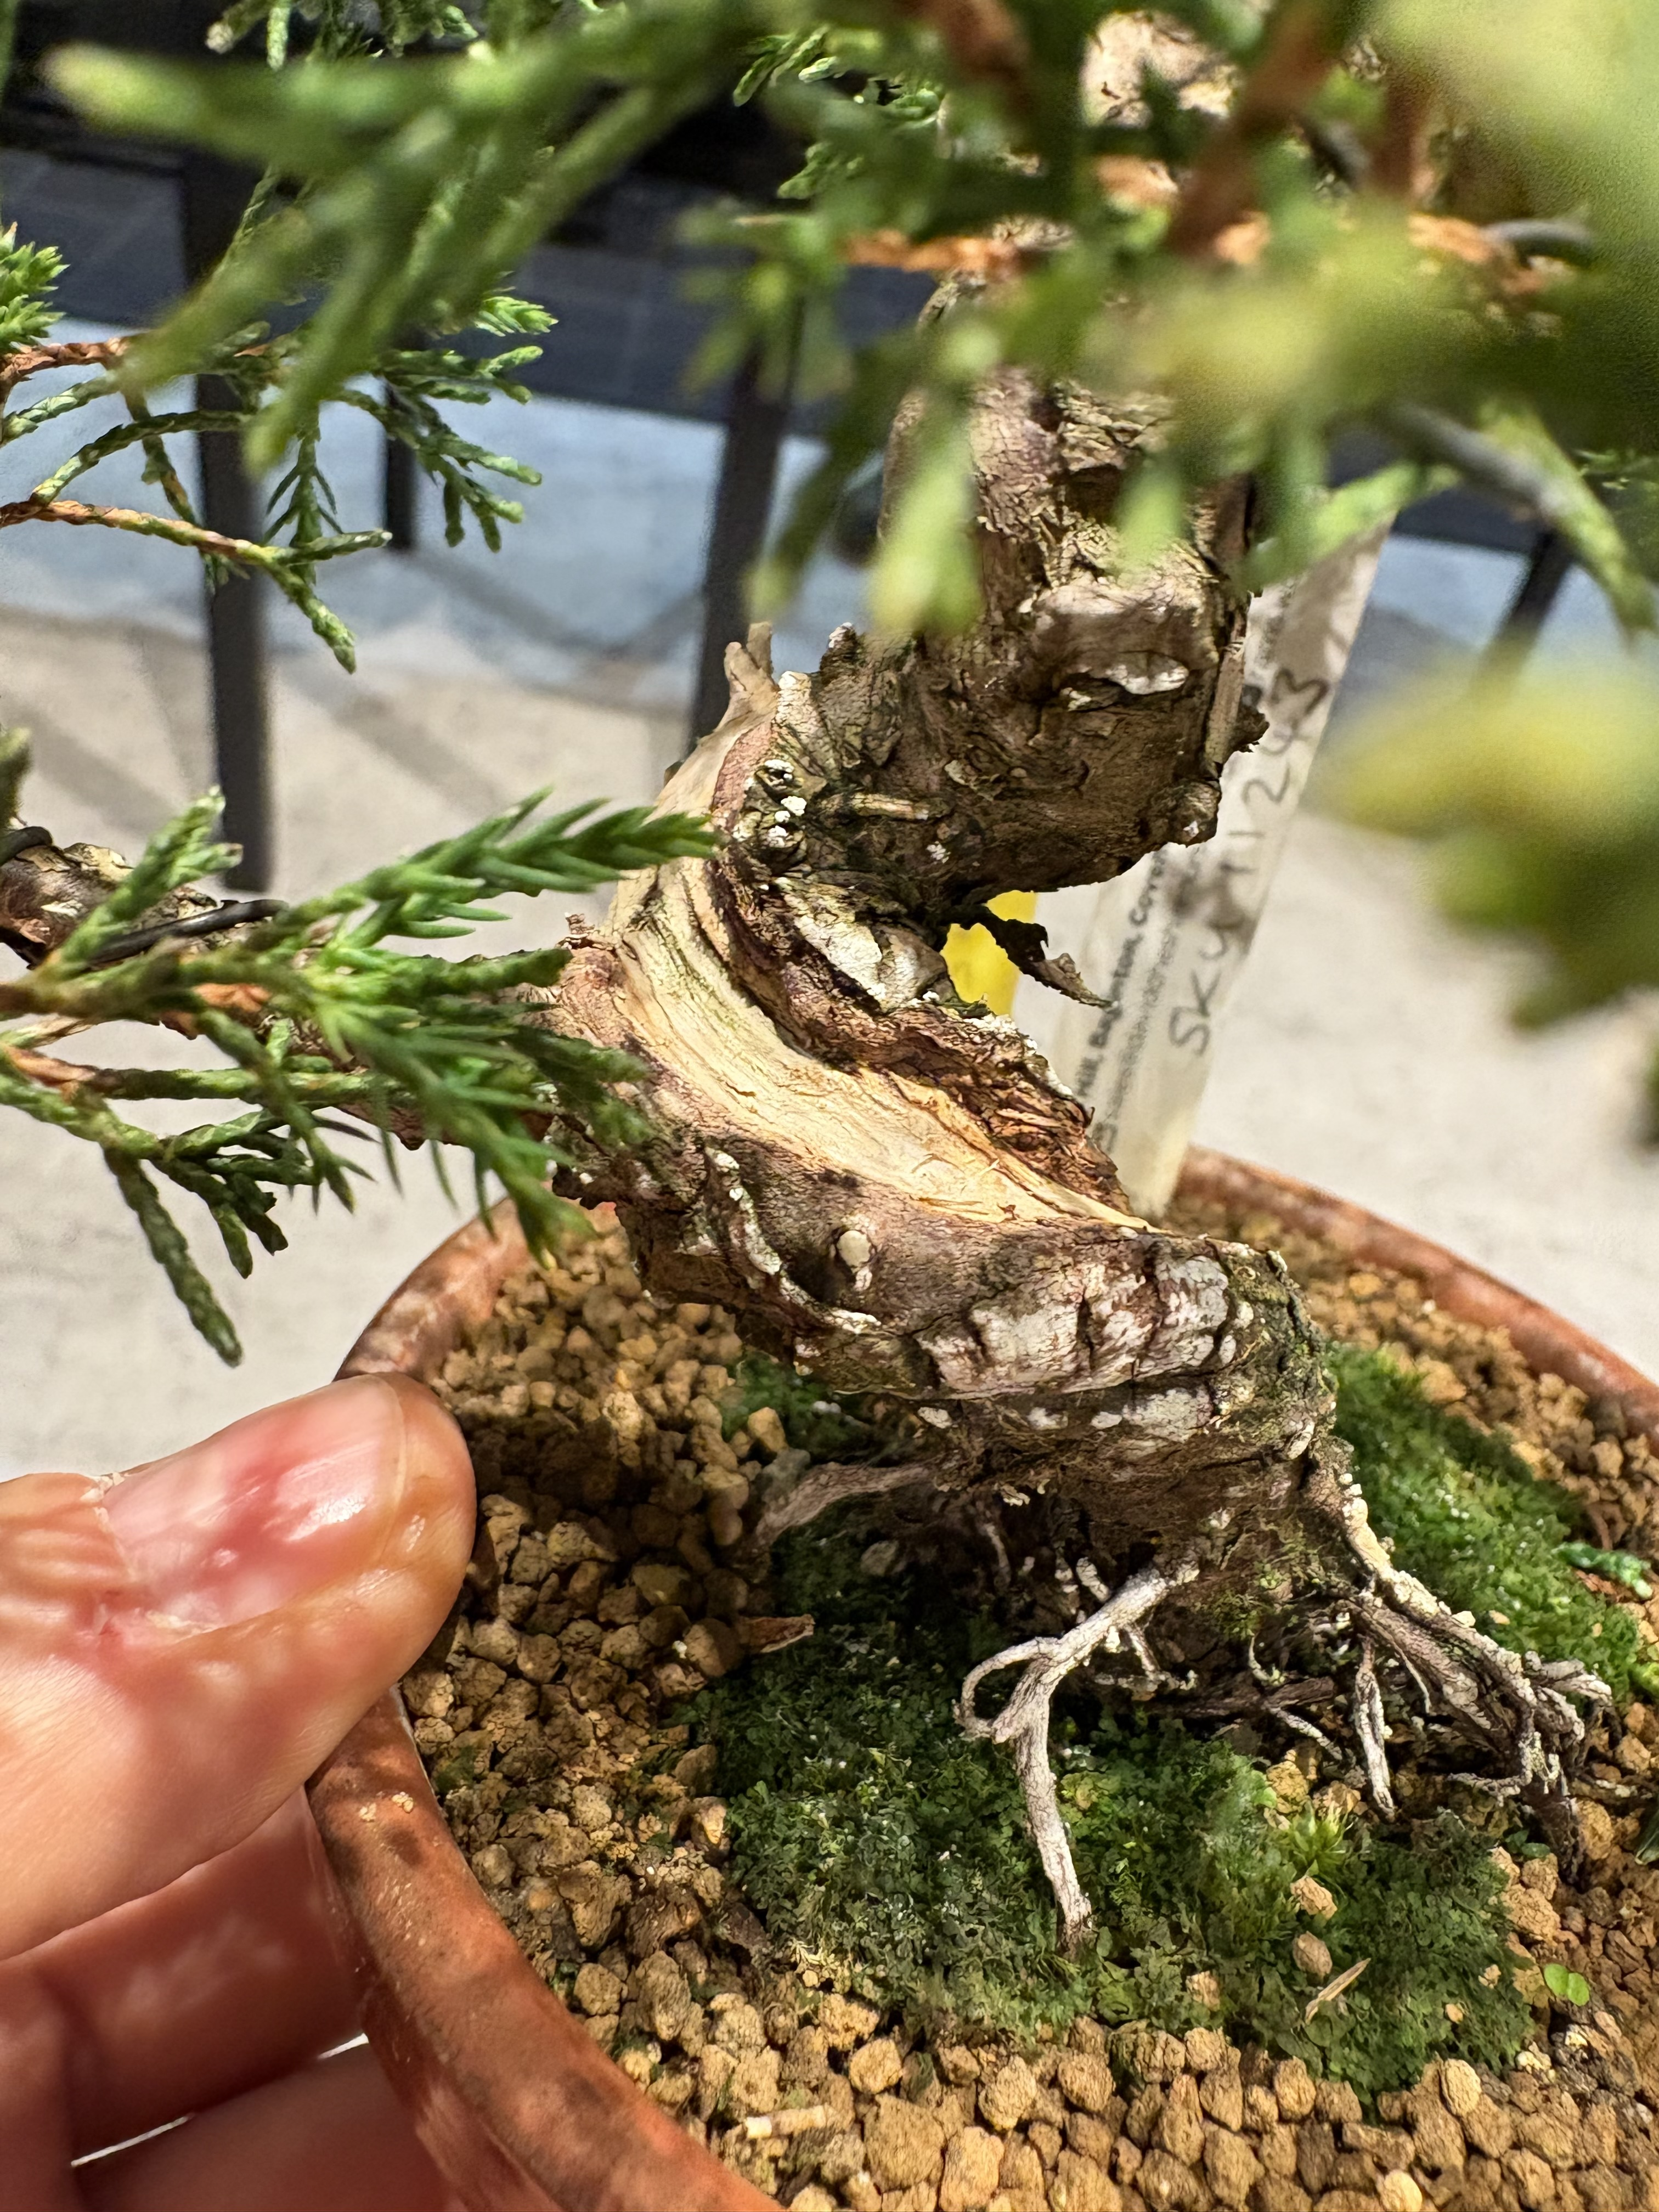
\includegraphics[angle=0,origin=c,width=1.0\textwidth]{2025_11/res/workshop_sebina_04.jpg}
\end{minipage}
\end{center}
\centerline{\emph{Examples of Sebina juniper bonsai from young cuttings.}}
\vfill
\clearpage

\begin{center}
\begin{minipage}[b]{.45\textwidth}
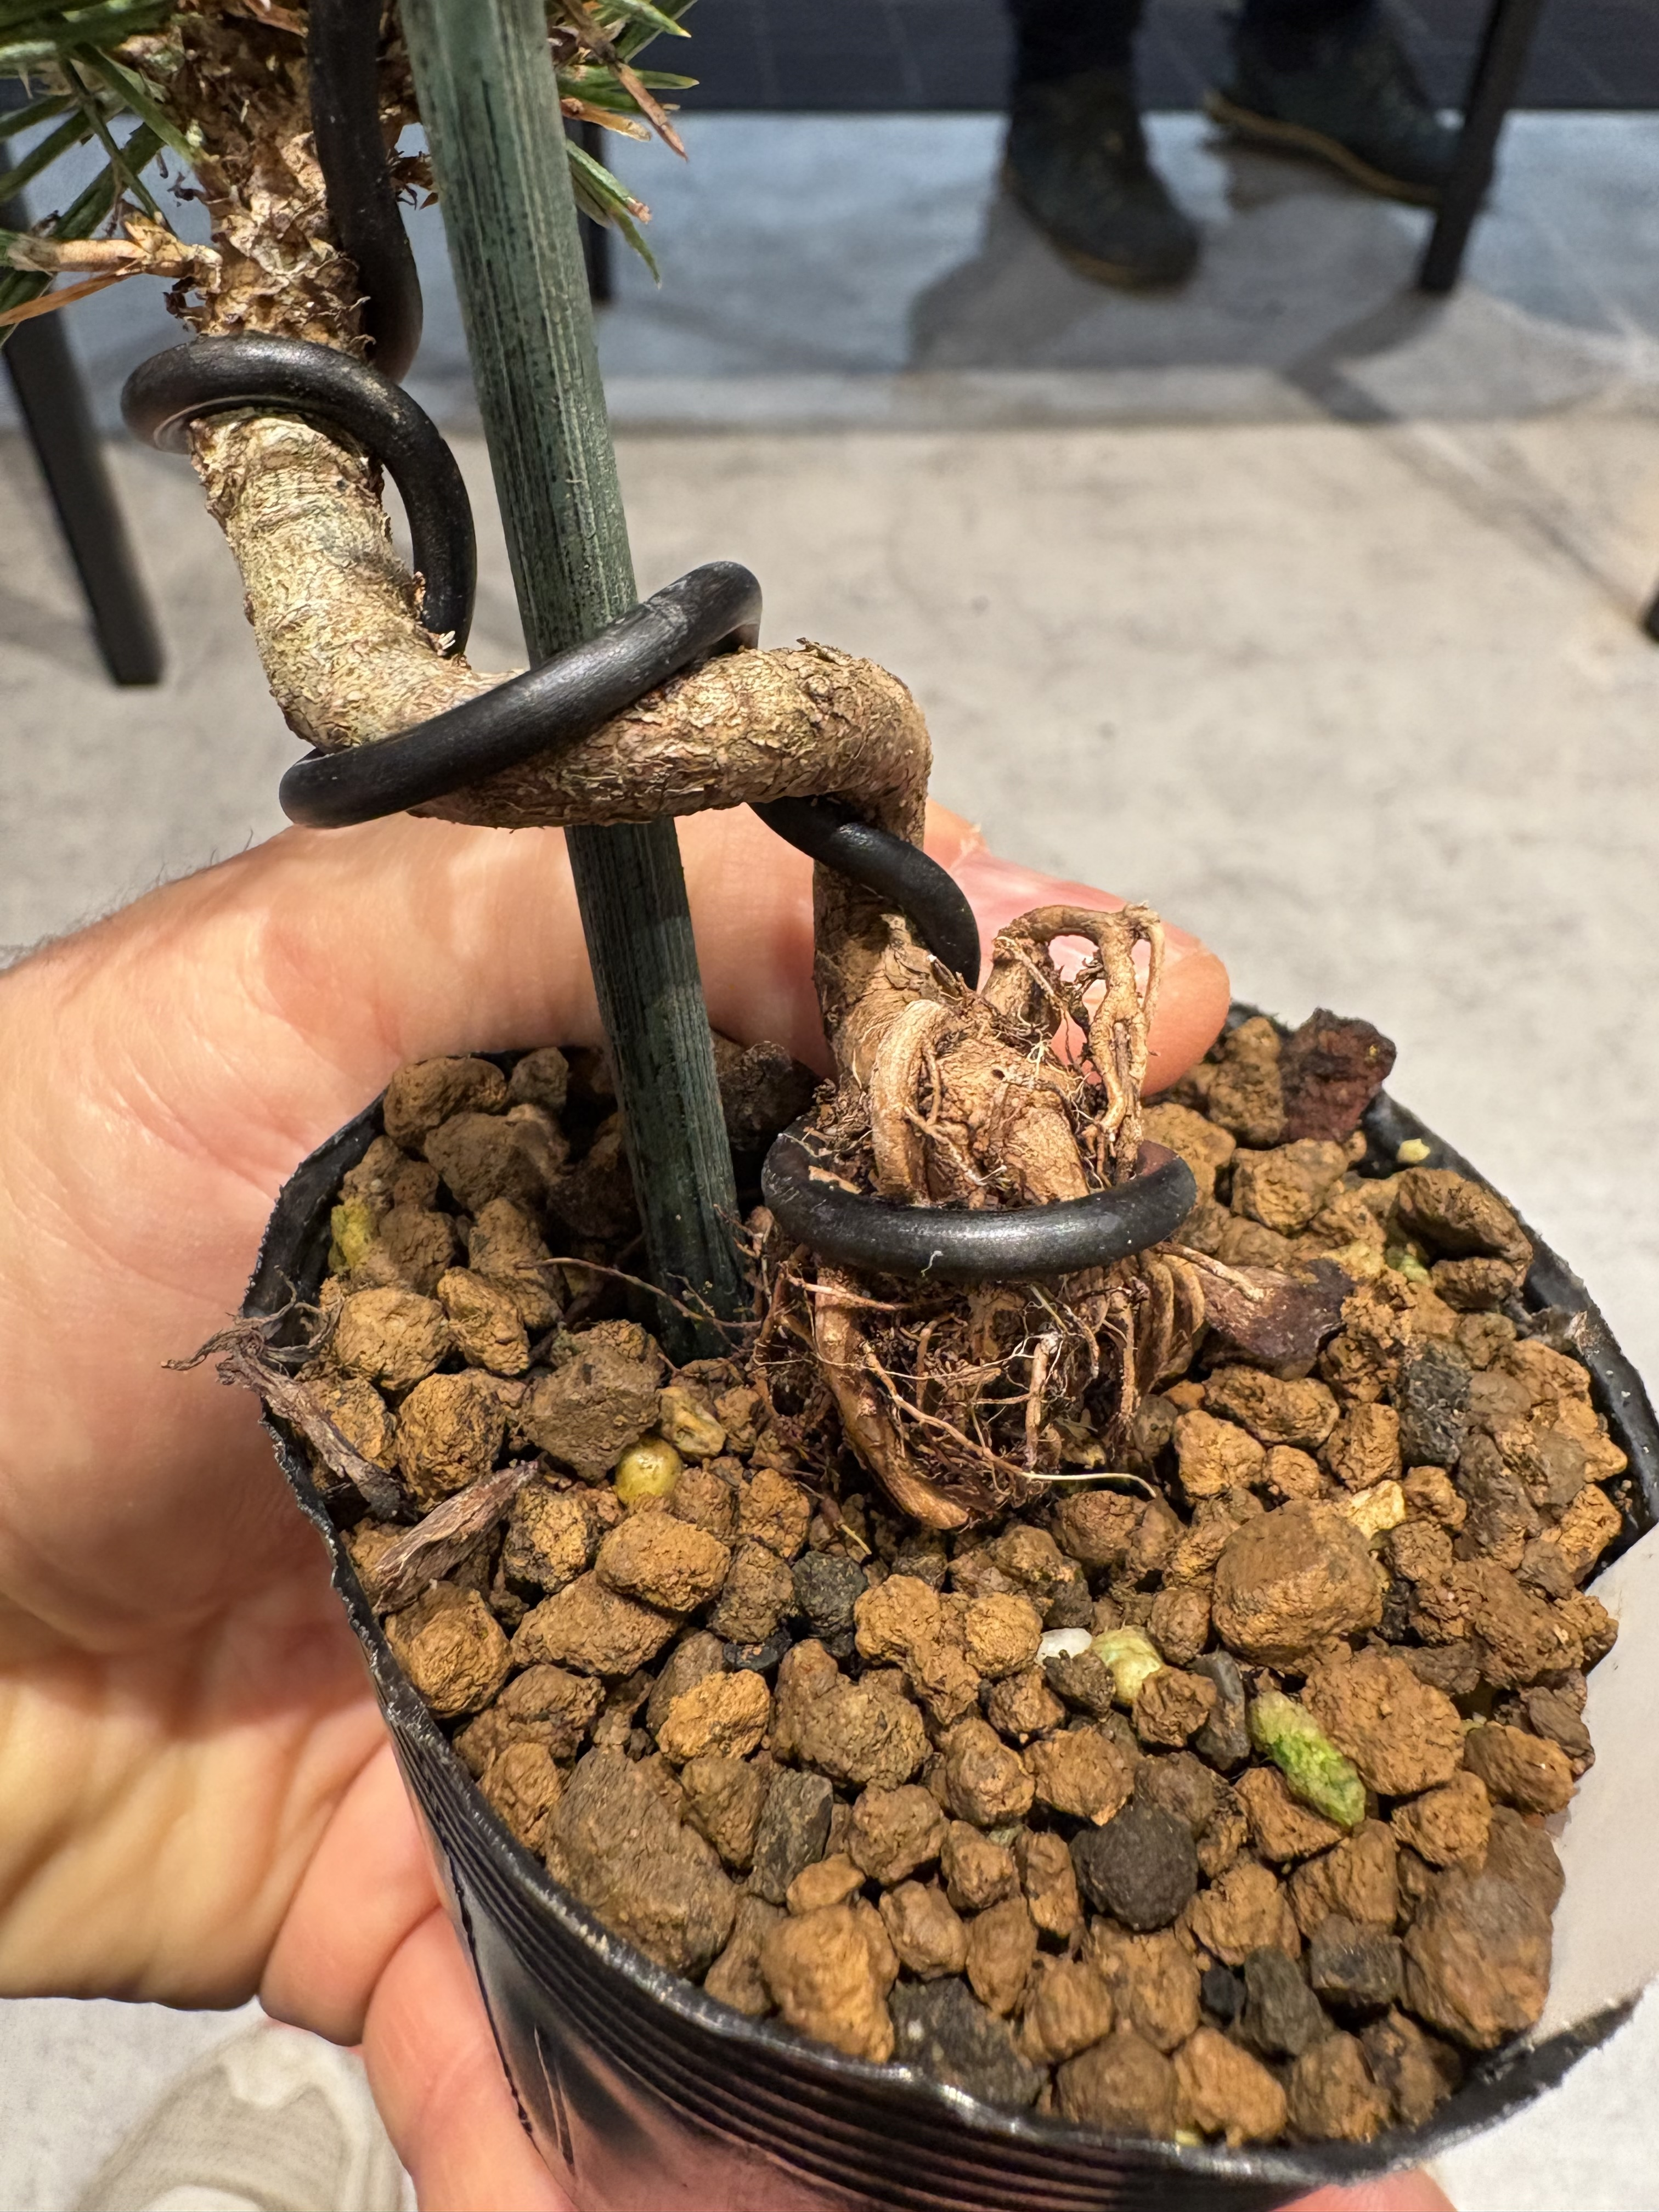
\includegraphics[angle=0,origin=c,width=1.0\textwidth]{2025_11/res/workshop_exposed_01.jpg}
\end{minipage}\quad
\begin{minipage}[b]{.45\textwidth}
\includegraphics[angle=0,origin=c,width=1.0\textwidth]{2025_11/res/workshop_exposed_02.jpg}
\end{minipage}
\medskip

\begin{minipage}[b]{.45\textwidth}
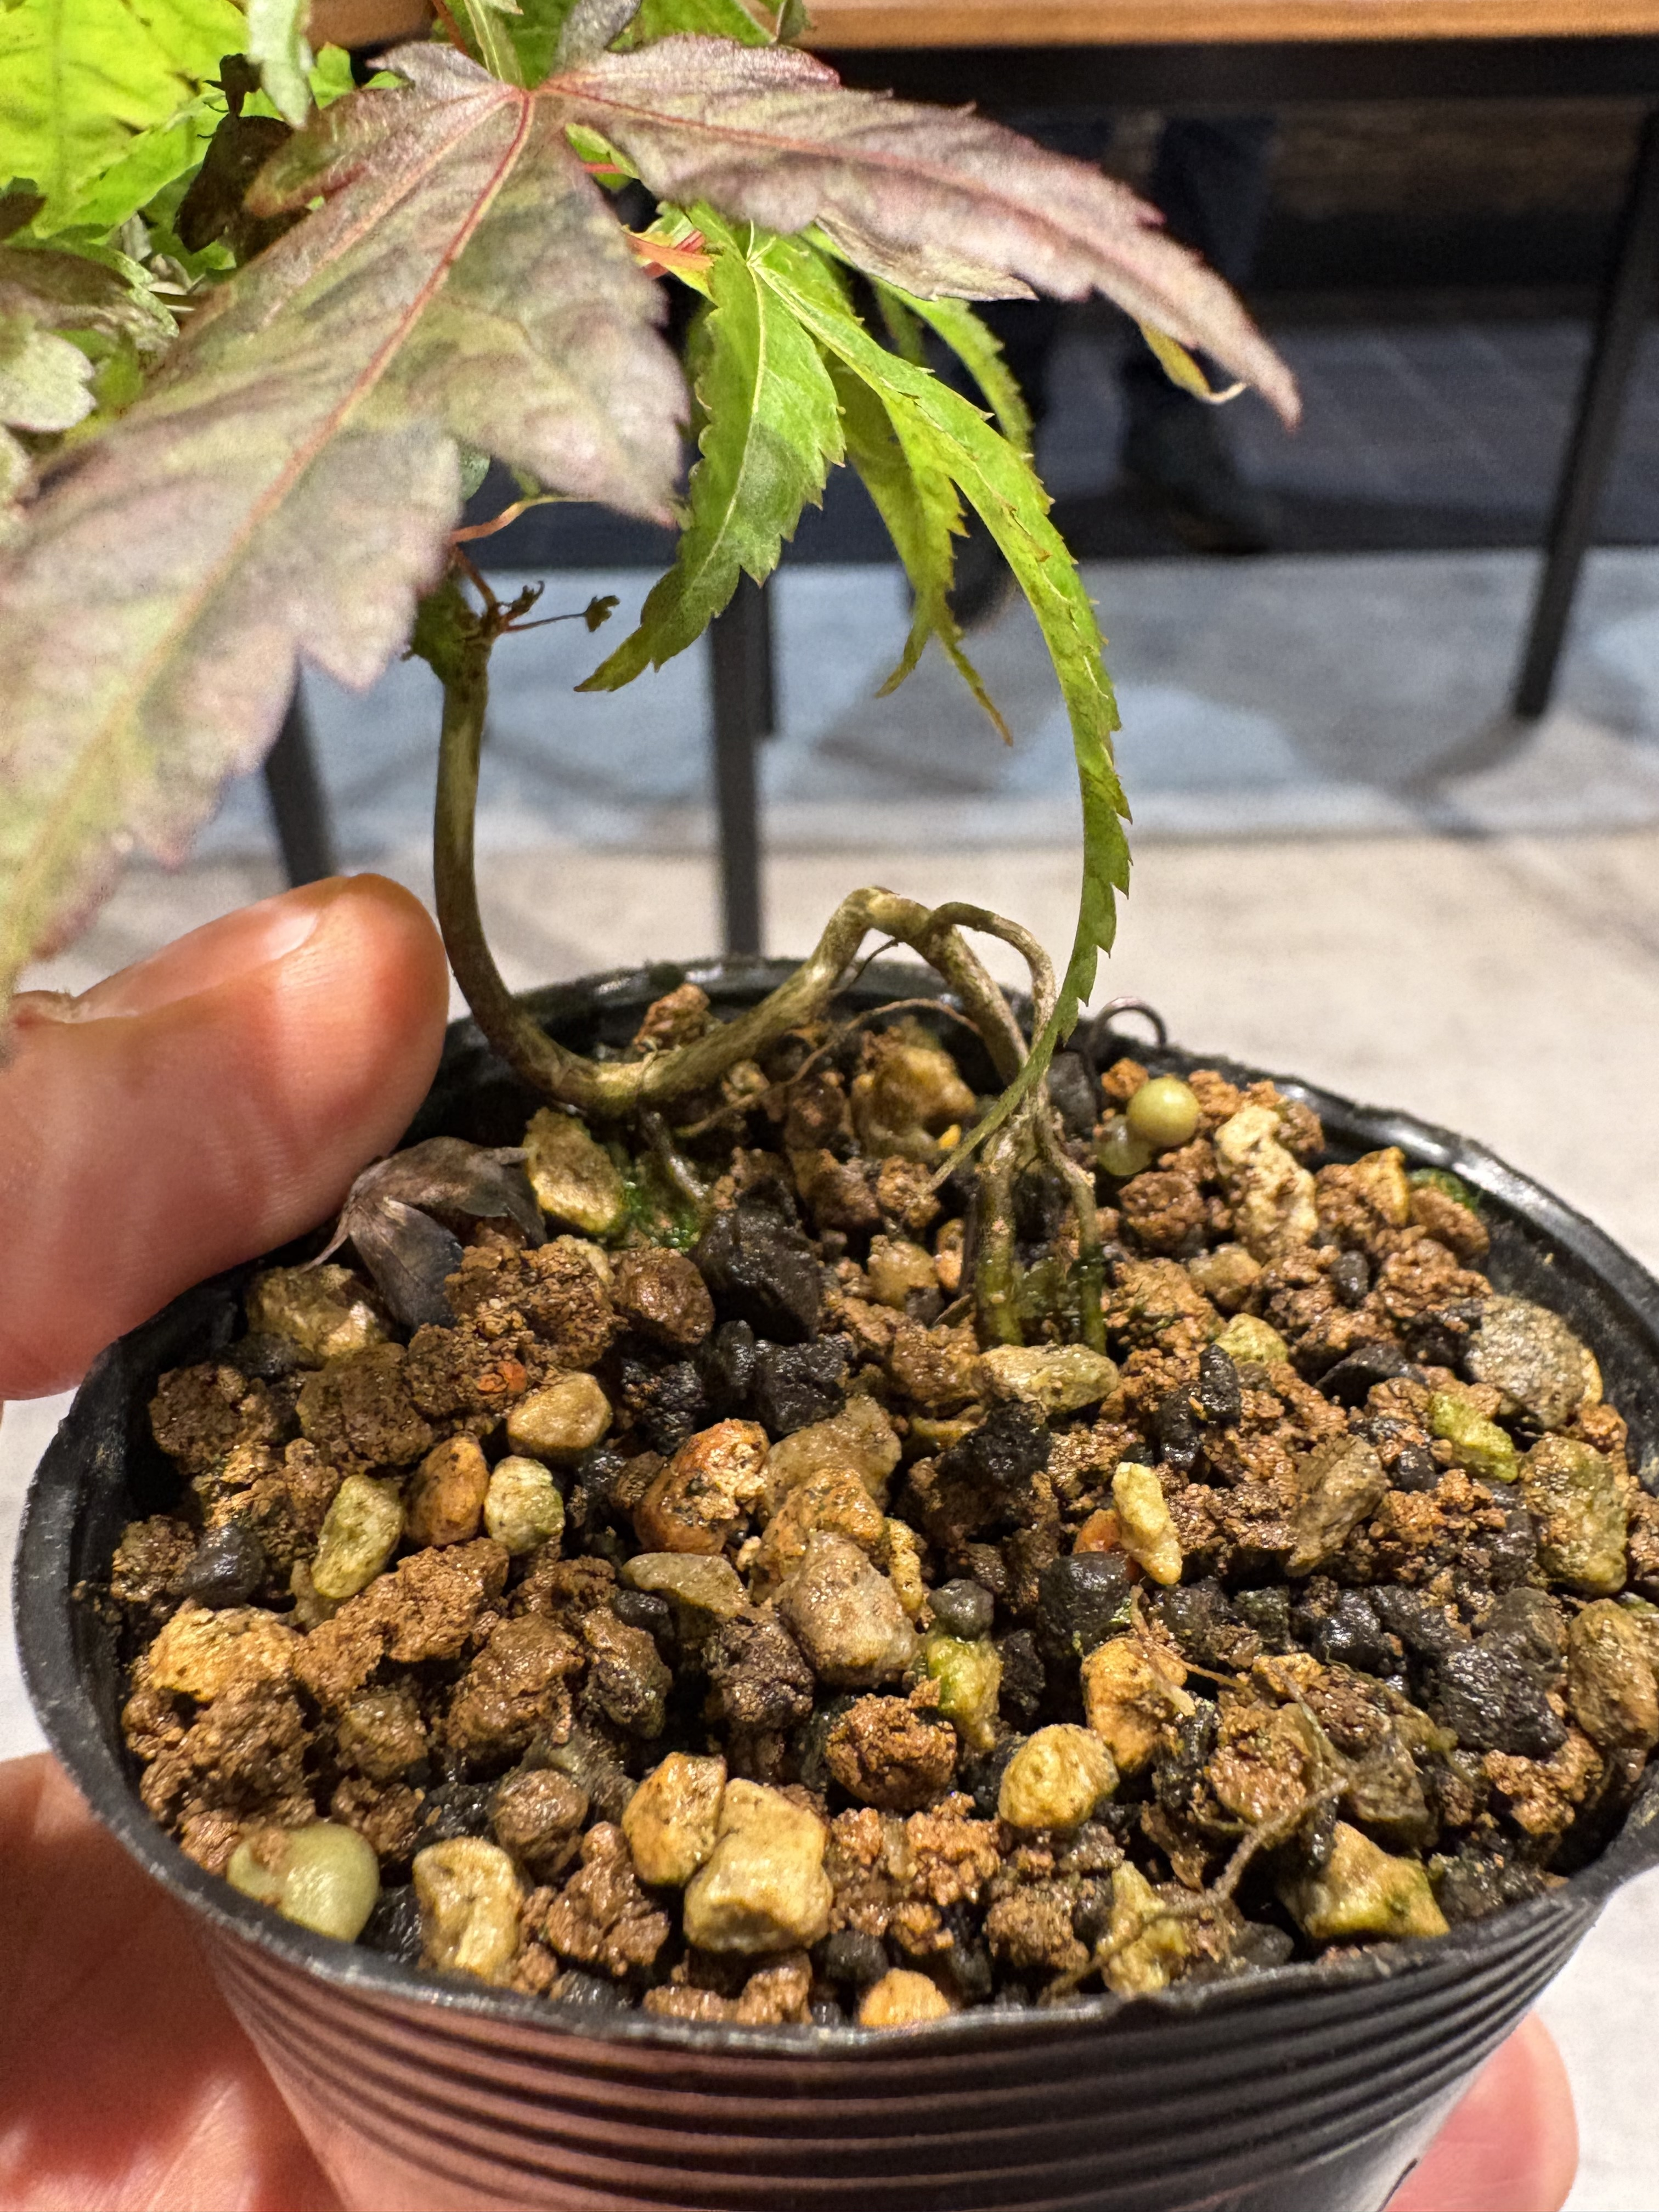
\includegraphics[angle=0,origin=c,width=1.0\textwidth]{2025_11/res/workshop_exposed_03.jpg}
\end{minipage}\quad
\begin{minipage}[b]{.45\textwidth}
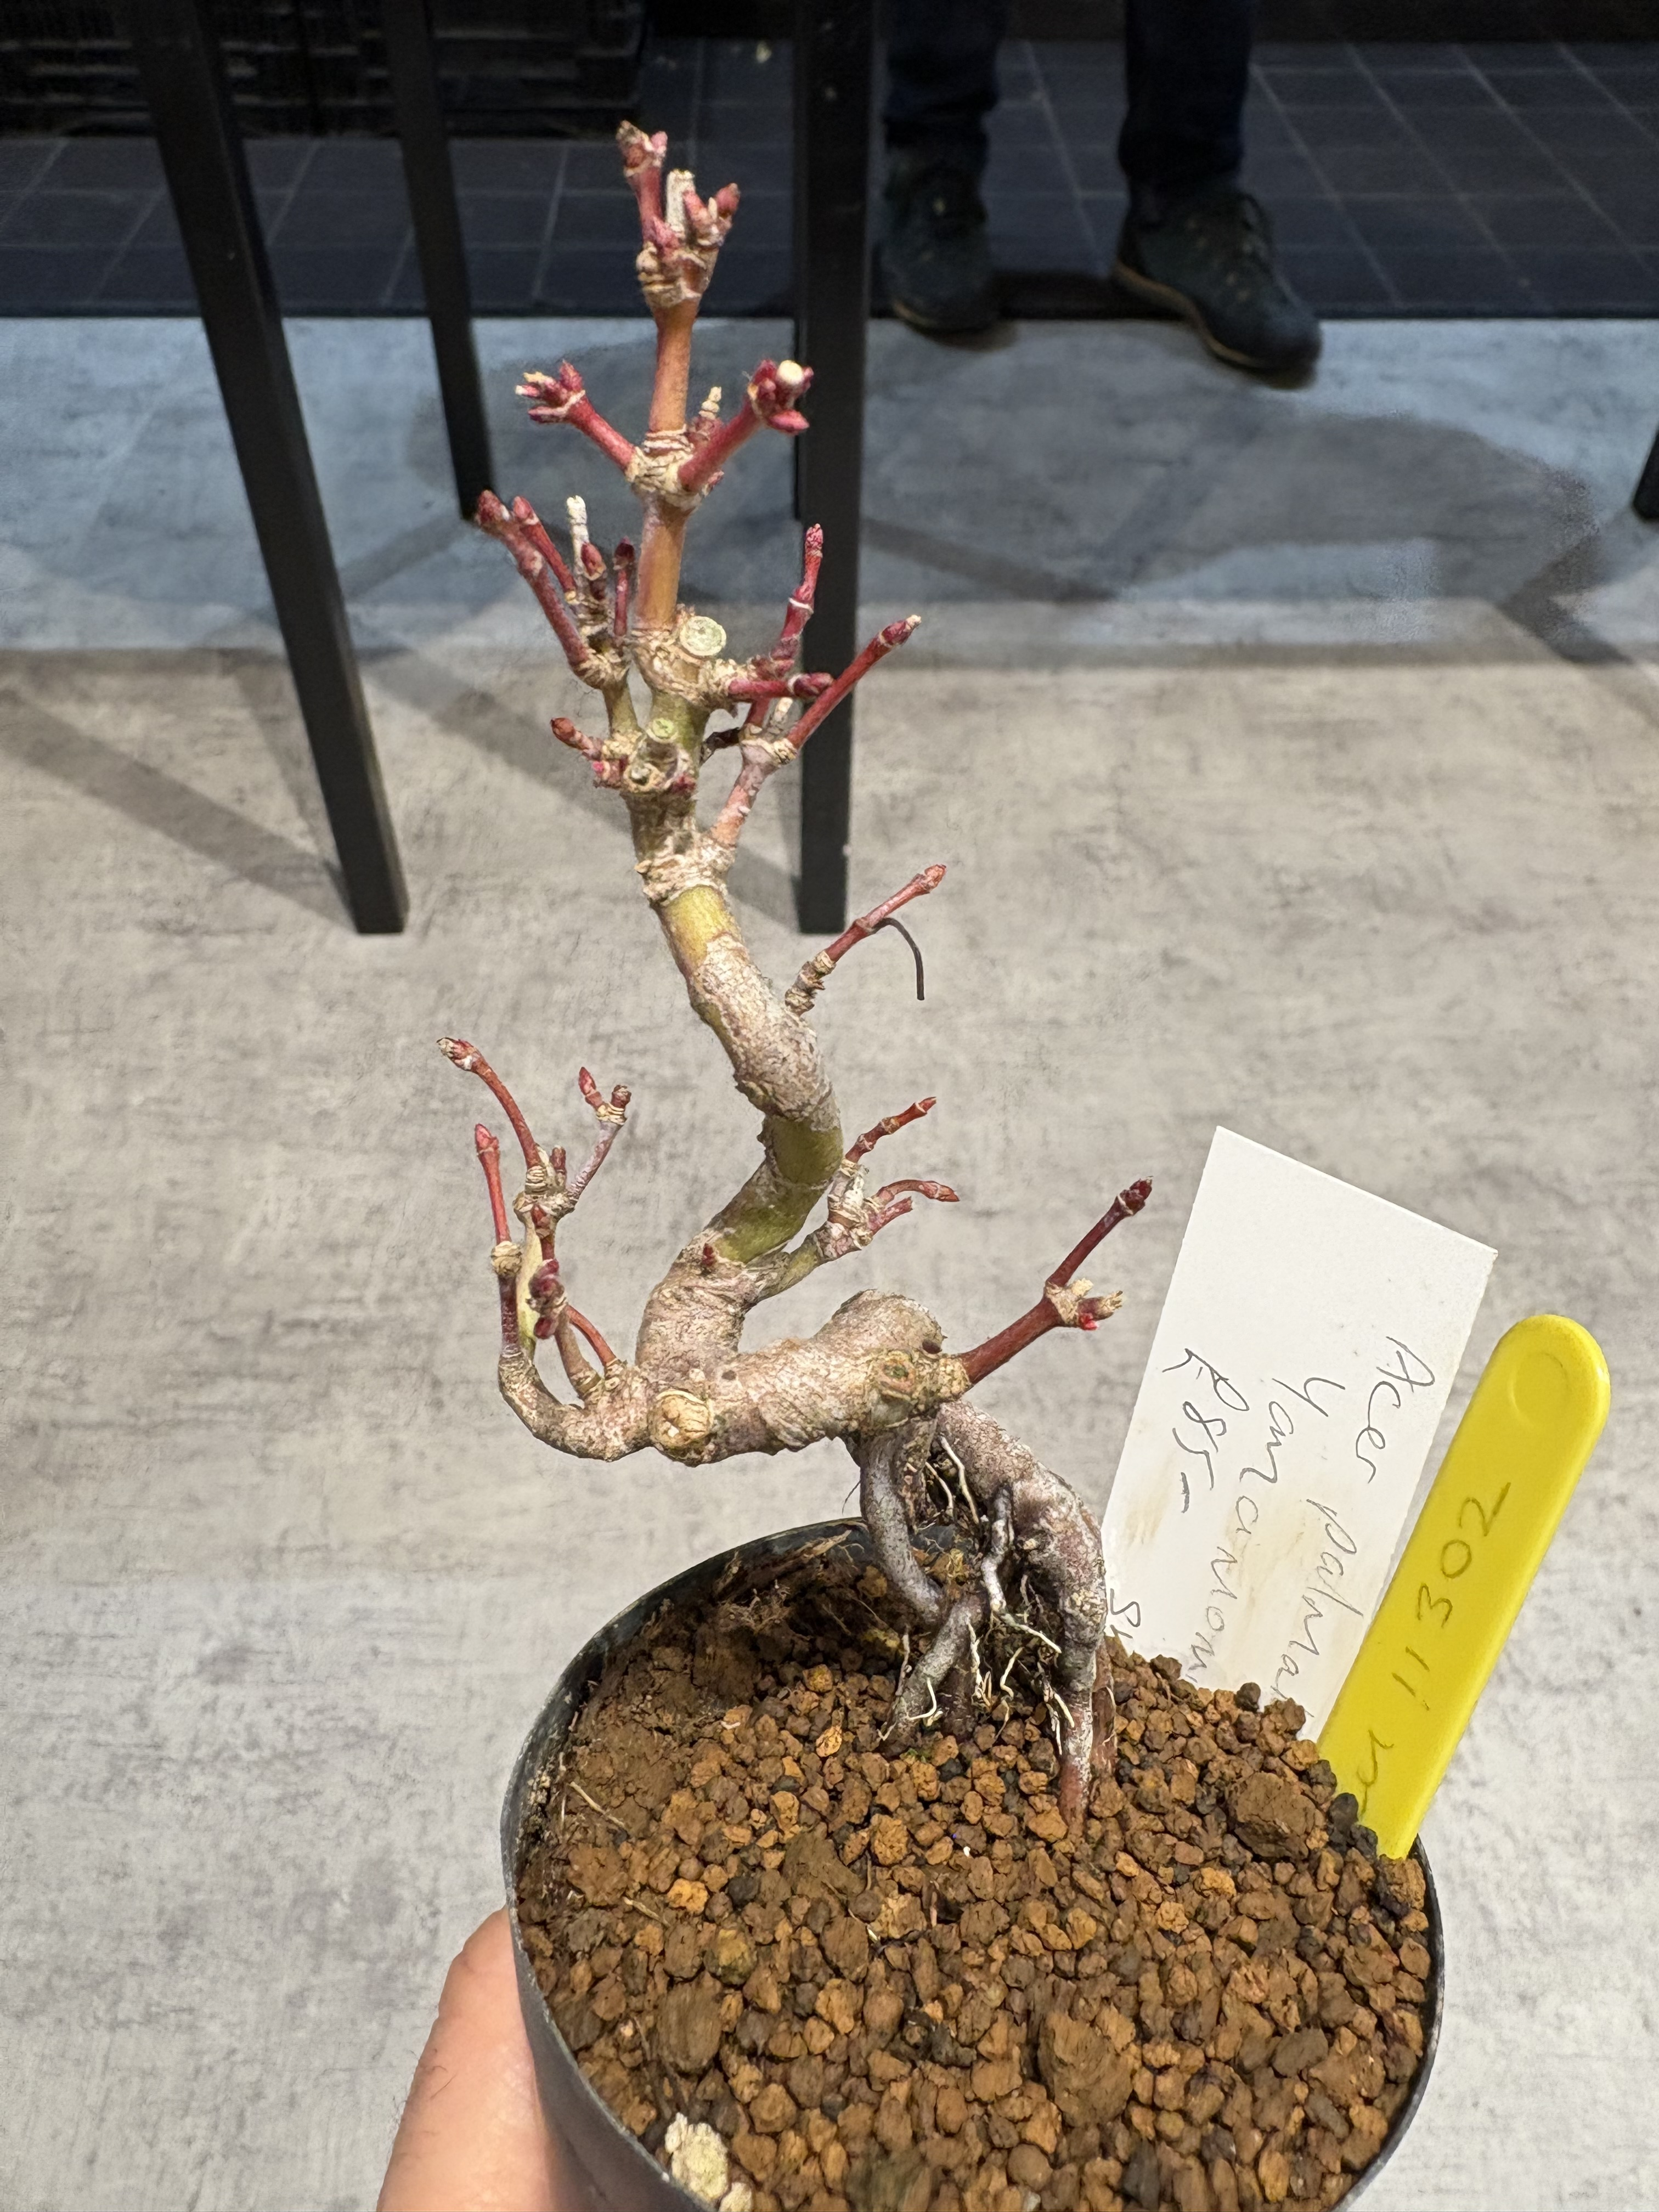
\includegraphics[angle=0,origin=c,width=1.0\textwidth]{2025_11/res/workshop_exposed_04.jpg}
\end{minipage}
\end{center}
\centerline{\emph{Progressively exposing pines and maples roots using moss tubes and wire.}}
\vfill
\clearpage

\begin{center}
\begin{minipage}[b]{.45\textwidth}
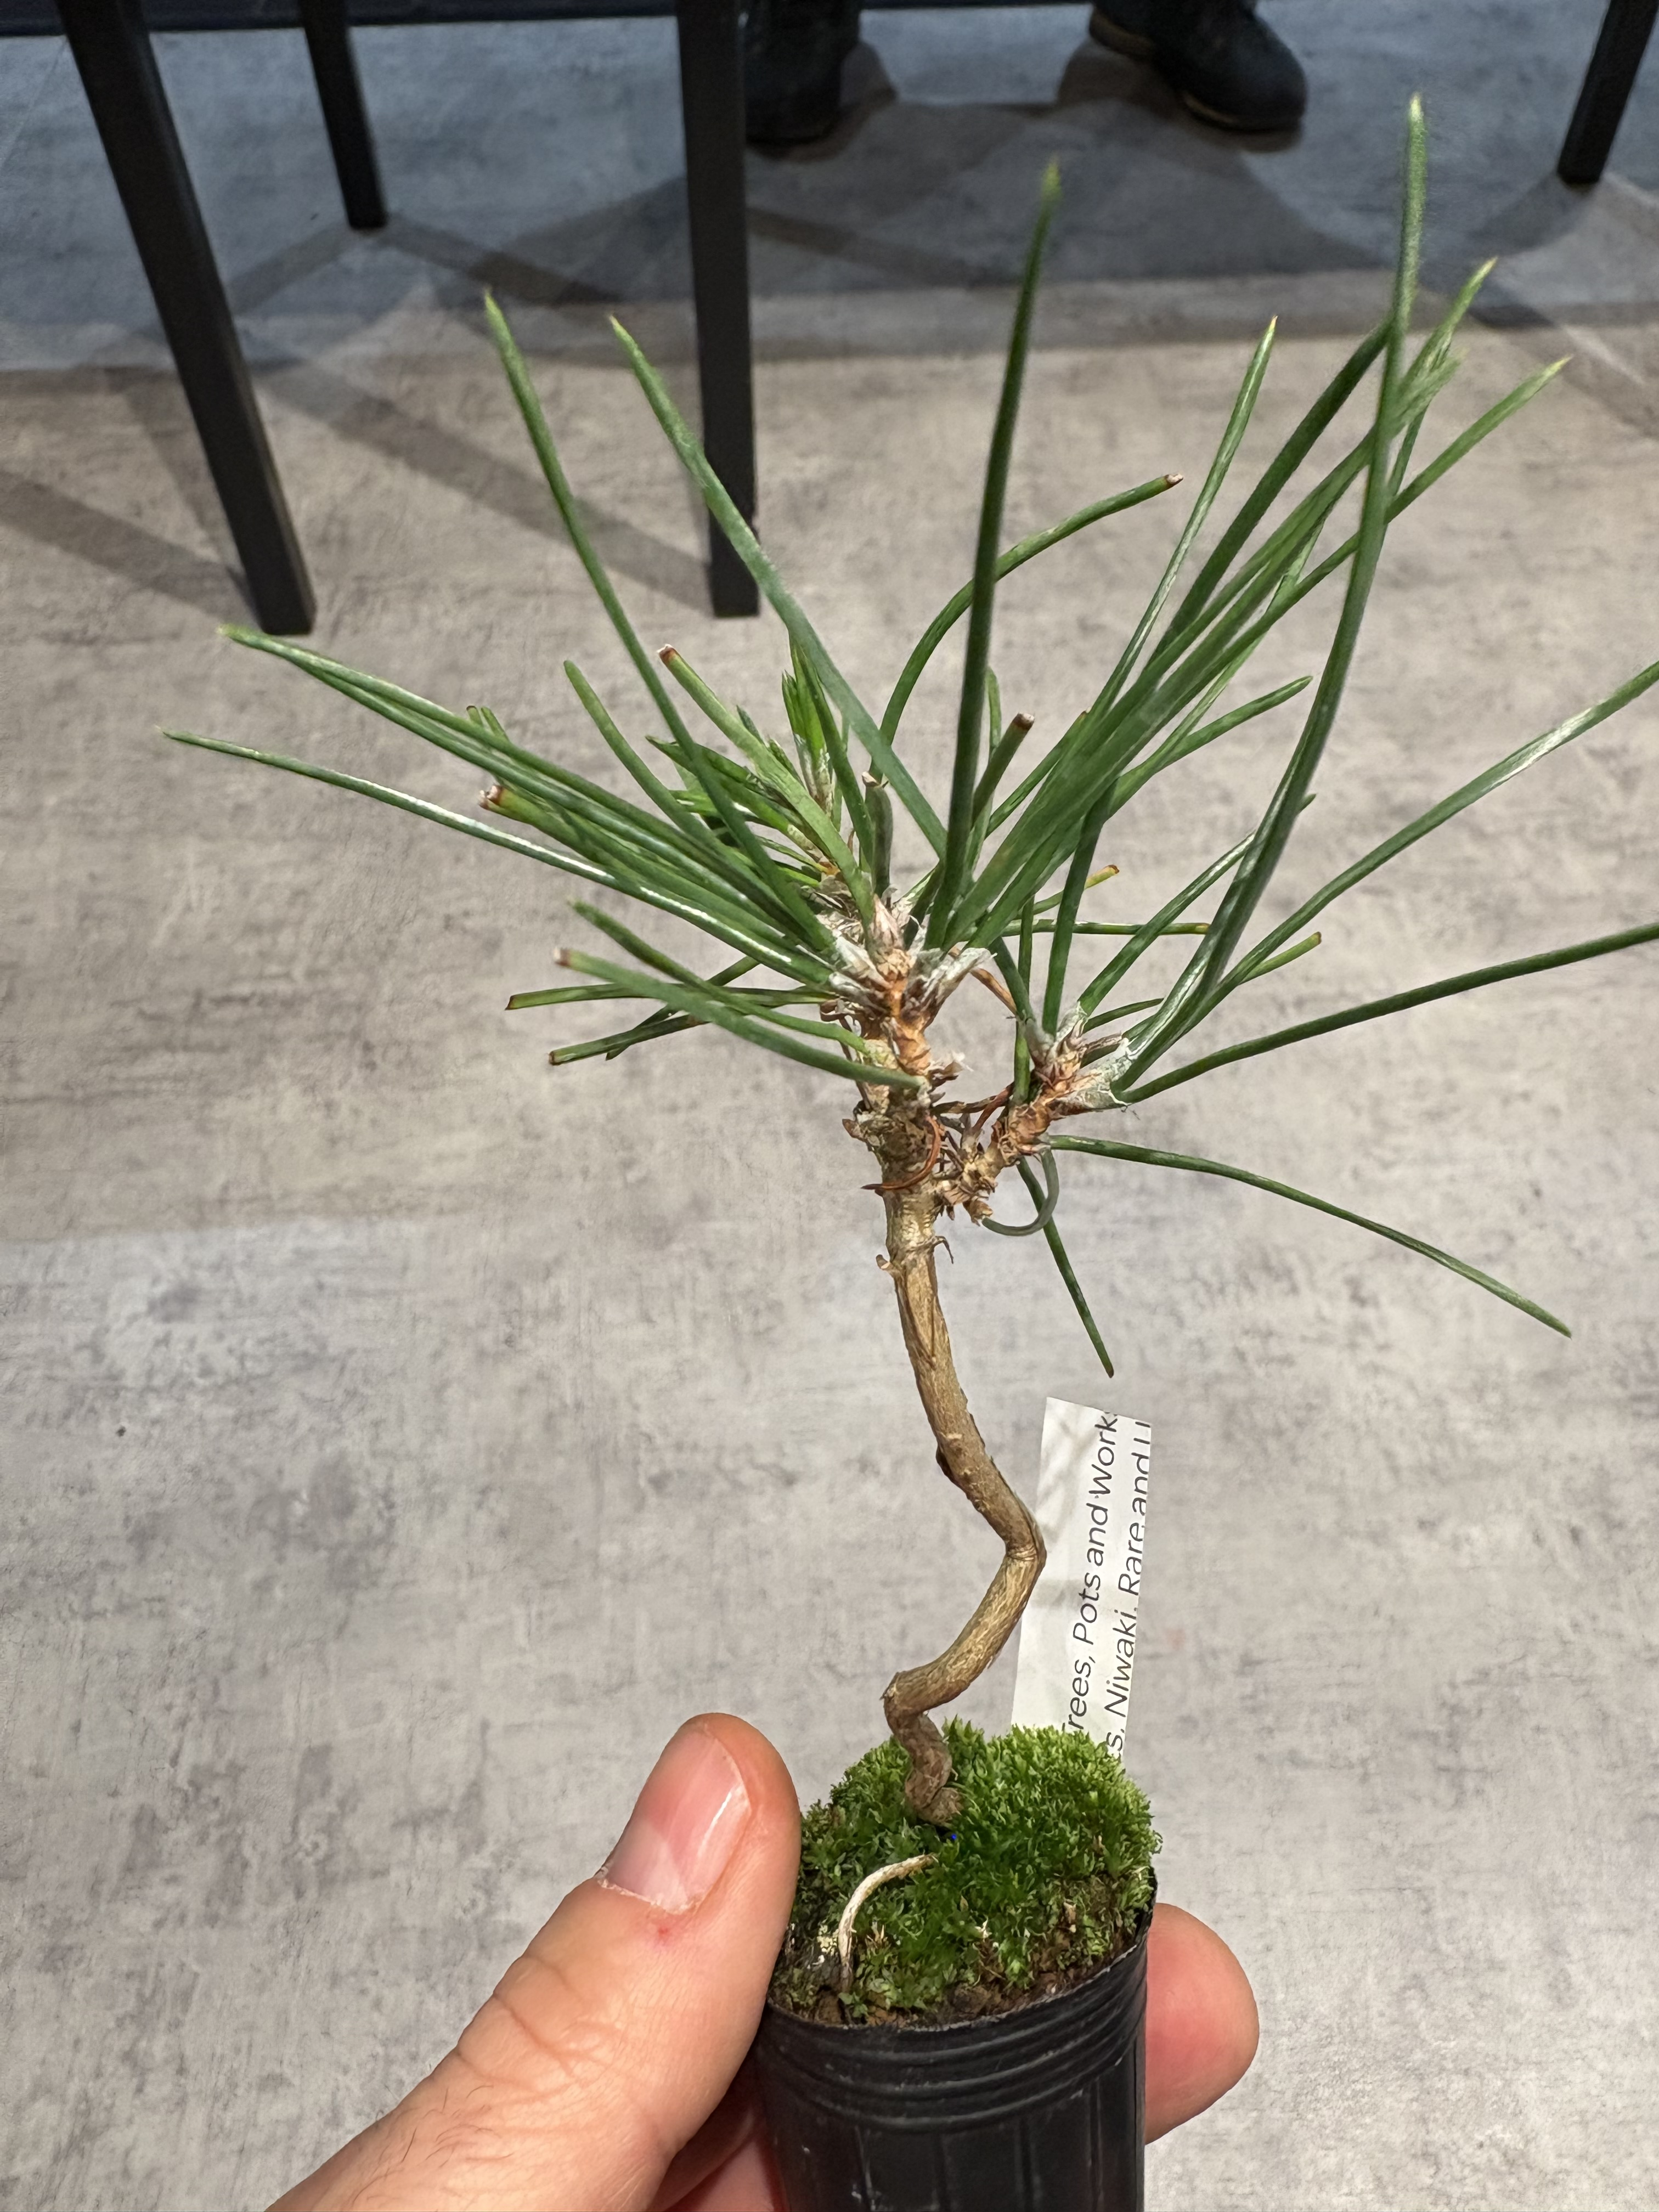
\includegraphics[angle=0,origin=c,width=1.0\textwidth]{2025_11/res/workshop_slow_01.jpg}
\end{minipage}\quad
\begin{minipage}[b]{.45\textwidth}
\includegraphics[angle=0,origin=c,width=1.0\textwidth]{2025_11/res/workshop_slow_02.jpg}
\end{minipage}
\medskip

\begin{minipage}[b]{.45\textwidth}
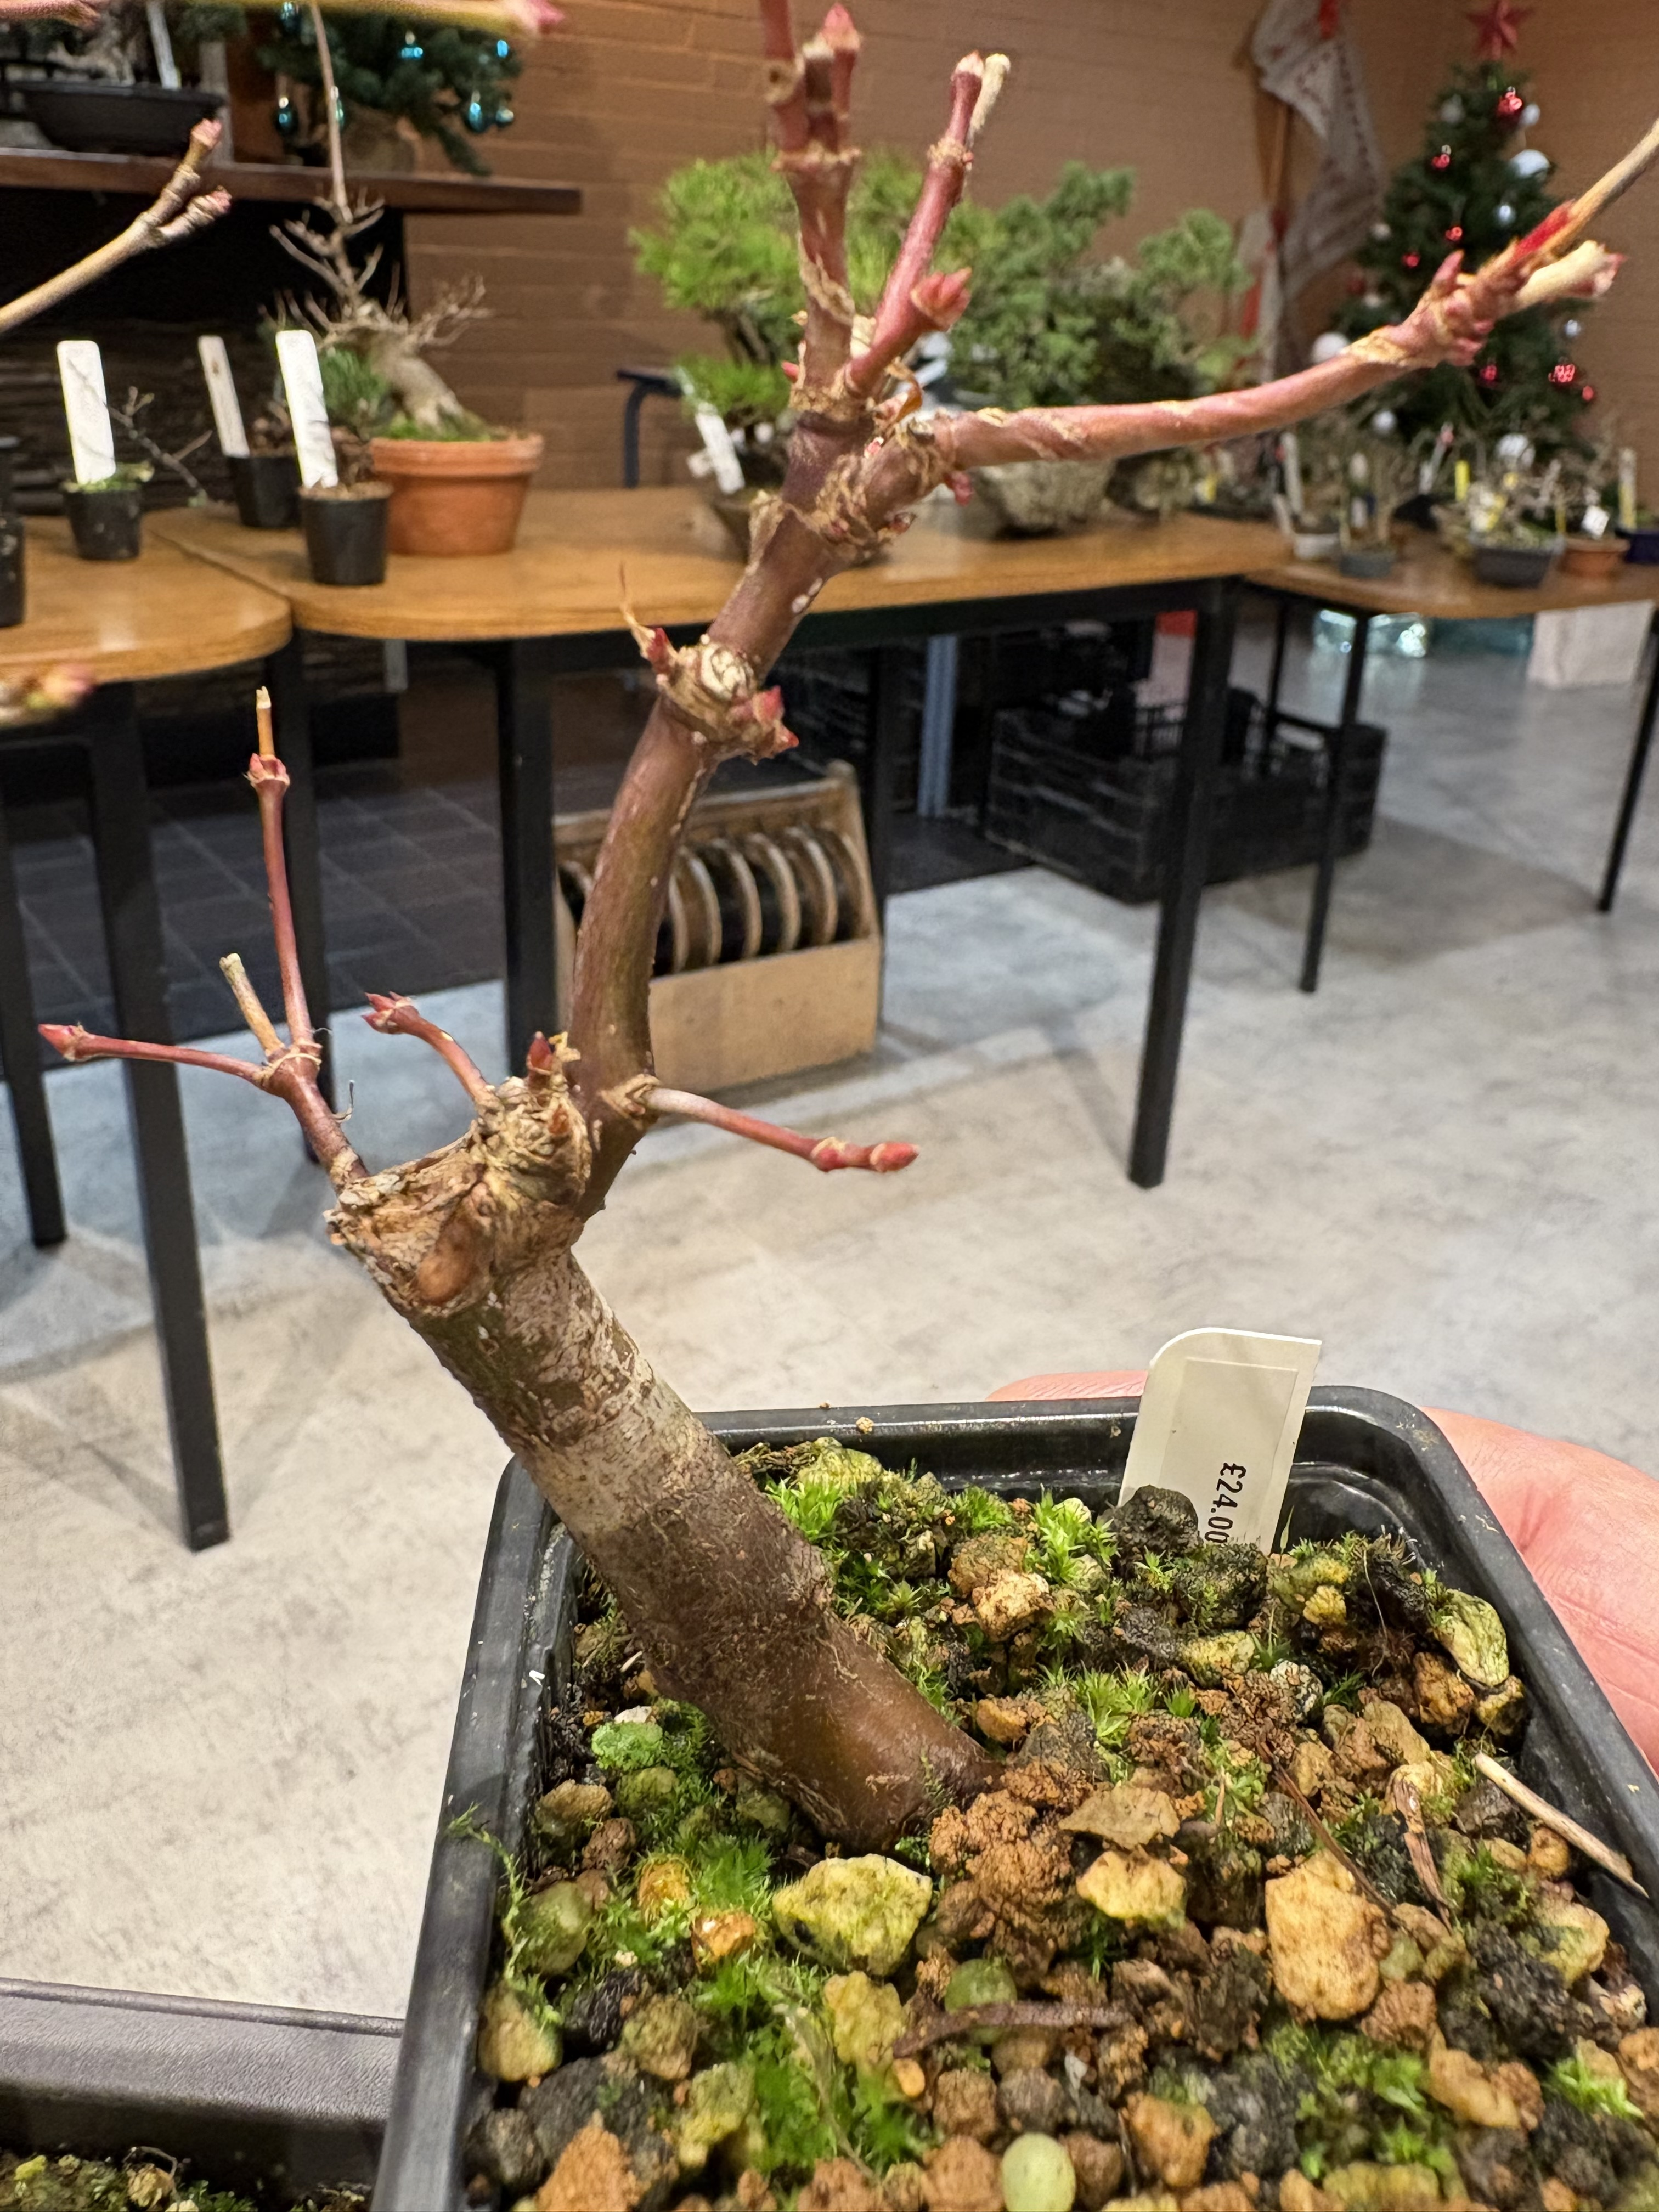
\includegraphics[angle=0,origin=c,width=1.0\textwidth]{2025_11/res/workshop_slow_03.jpg}
\end{minipage}\quad
\begin{minipage}[b]{.45\textwidth}
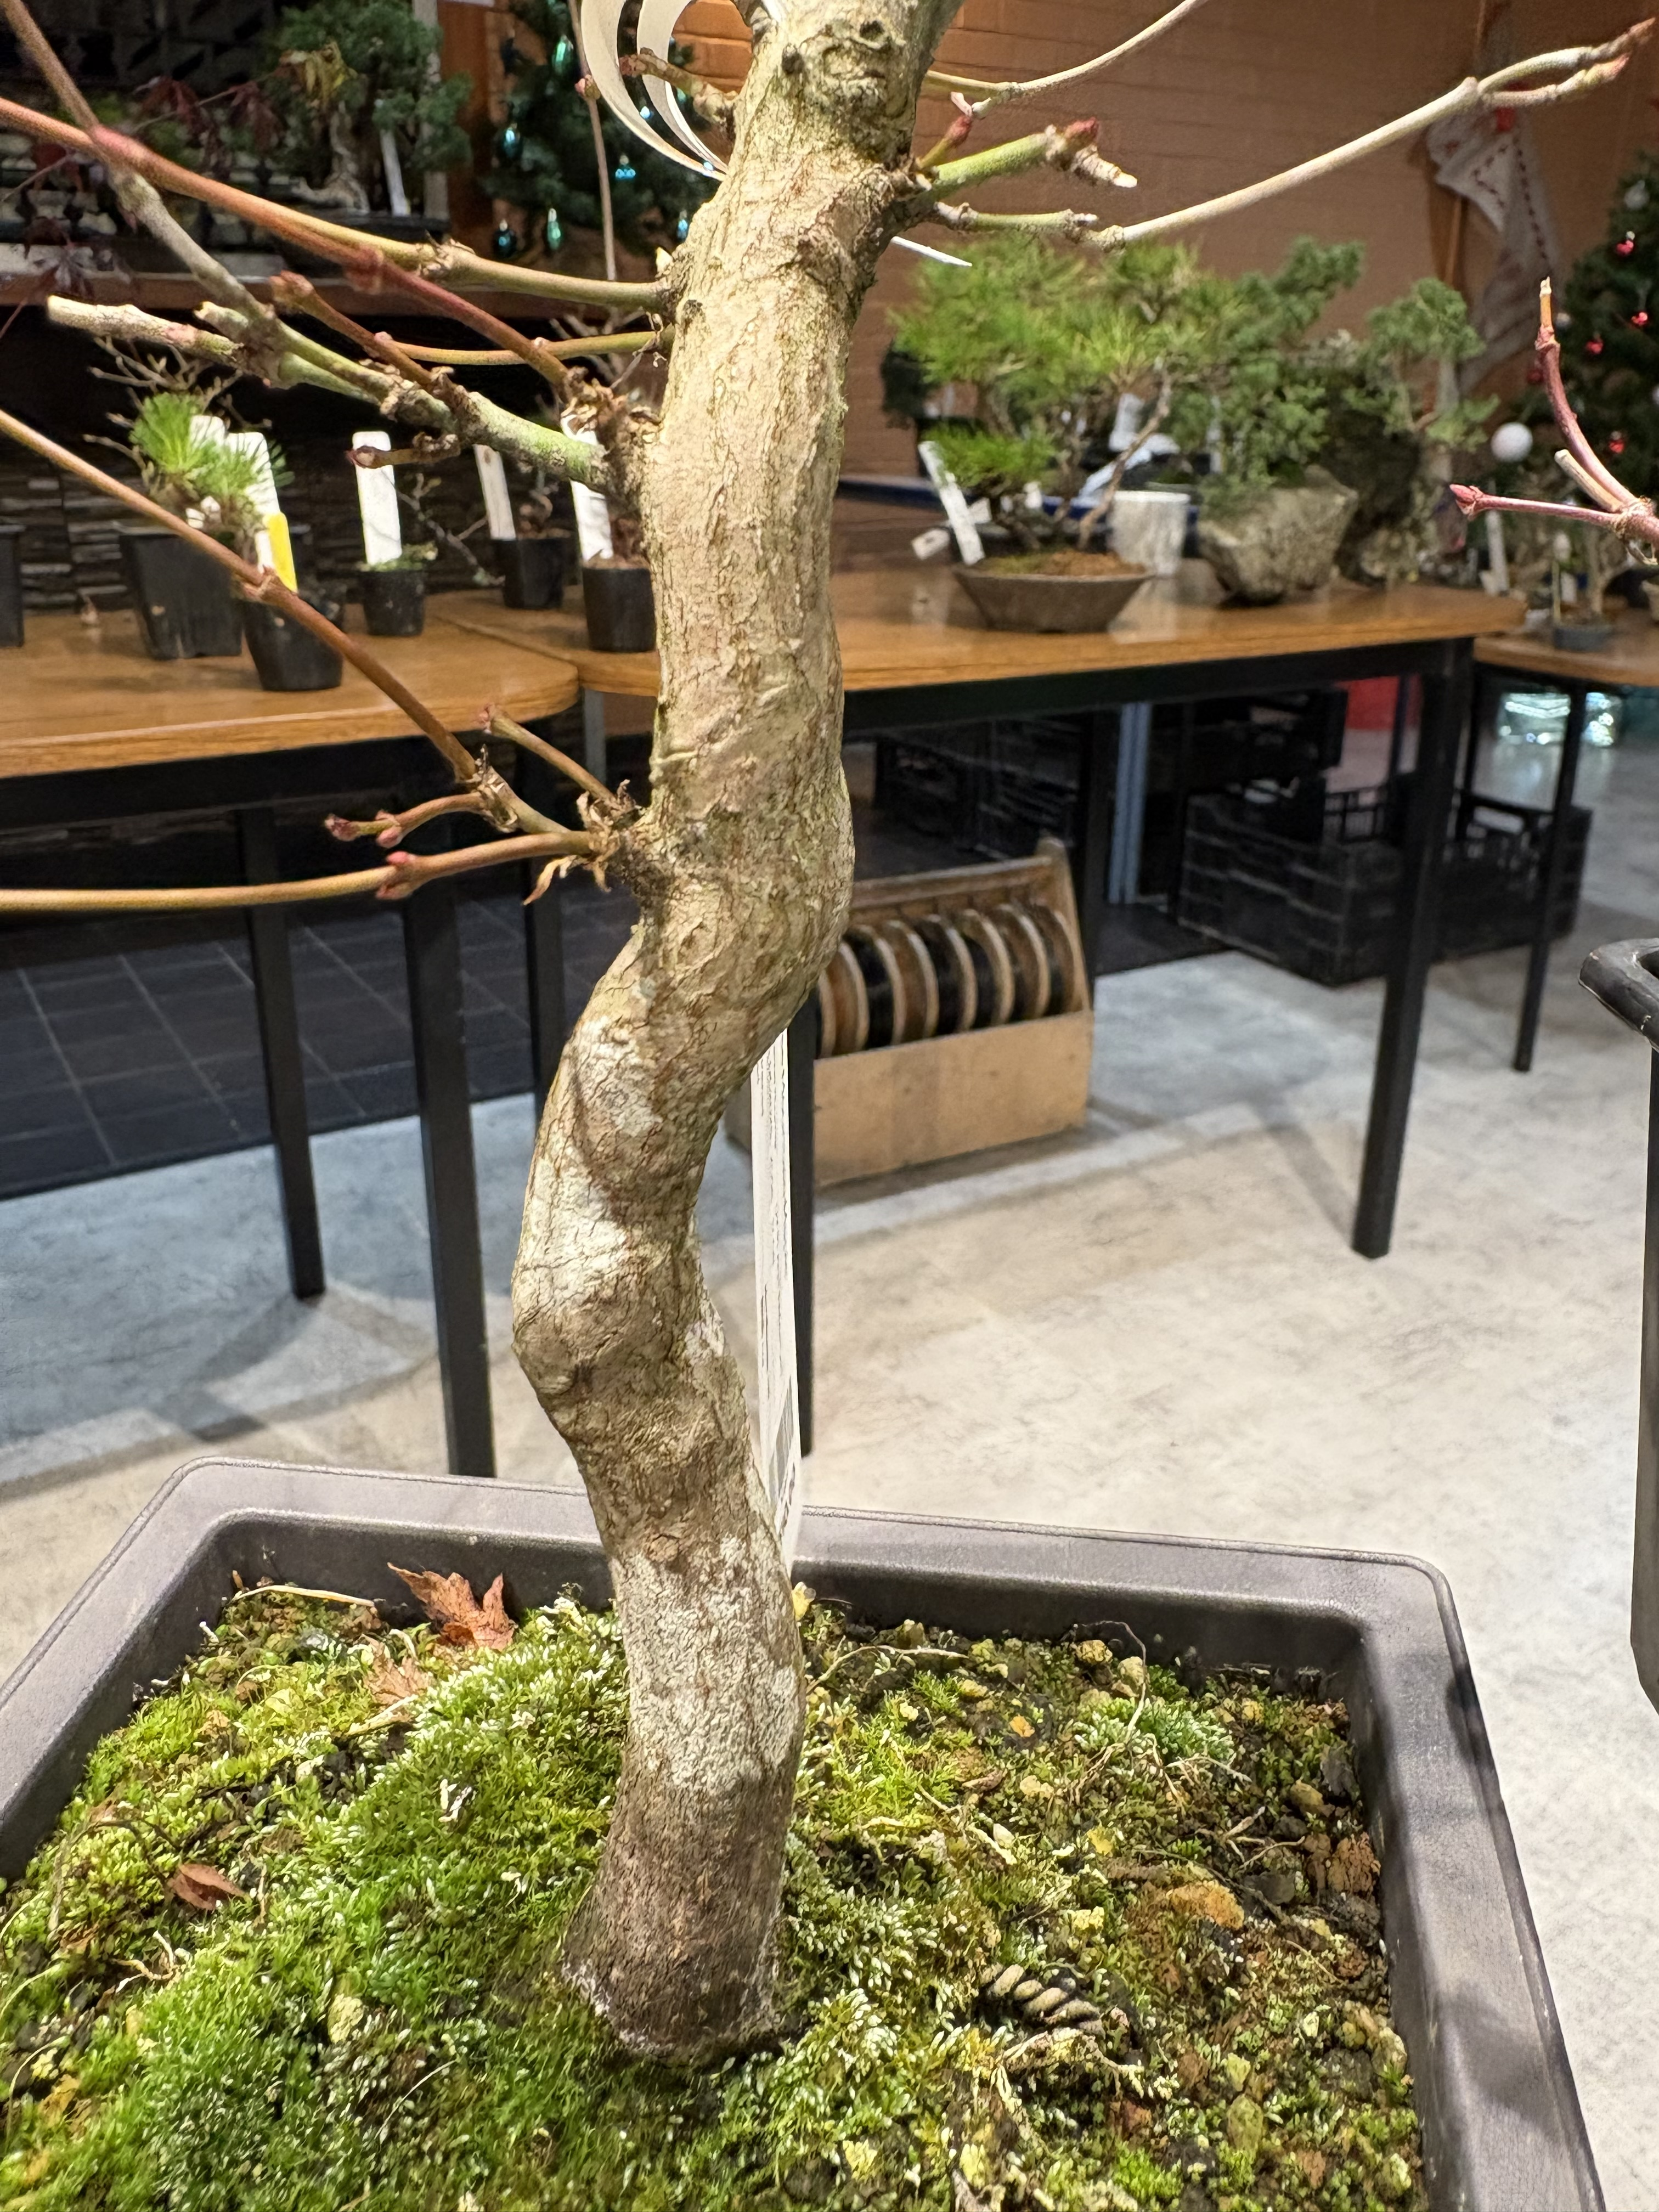
\includegraphics[angle=0,origin=c,width=1.0\textwidth]{2025_11/res/workshop_slow_04.jpg}
\end{minipage}
\end{center}
\centerline{\emph{Slow early growth—followed by rapid spurts in pines—helps maple and pine bark mature beautifully.}}
\vfill
\clearpage

\begin{center}
\begin{minipage}[b]{.45\textwidth}
\includegraphics[angle=0,origin=c,width=1.0\textwidth]{2025_11/res/workshop_grafting_01.jpg}
\end{minipage}\quad
\begin{minipage}[b]{.45\textwidth}
\includegraphics[angle=0,origin=c,width=1.0\textwidth]{2025_11/res/workshop_grafting_02.jpg}
\end{minipage}
\medskip

\begin{minipage}[b]{.45\textwidth}
\includegraphics[angle=0,origin=c,width=1.0\textwidth]{2025_11/res/workshop_sacrifice_01.jpg}
\end{minipage}\quad
\begin{minipage}[b]{.45\textwidth}
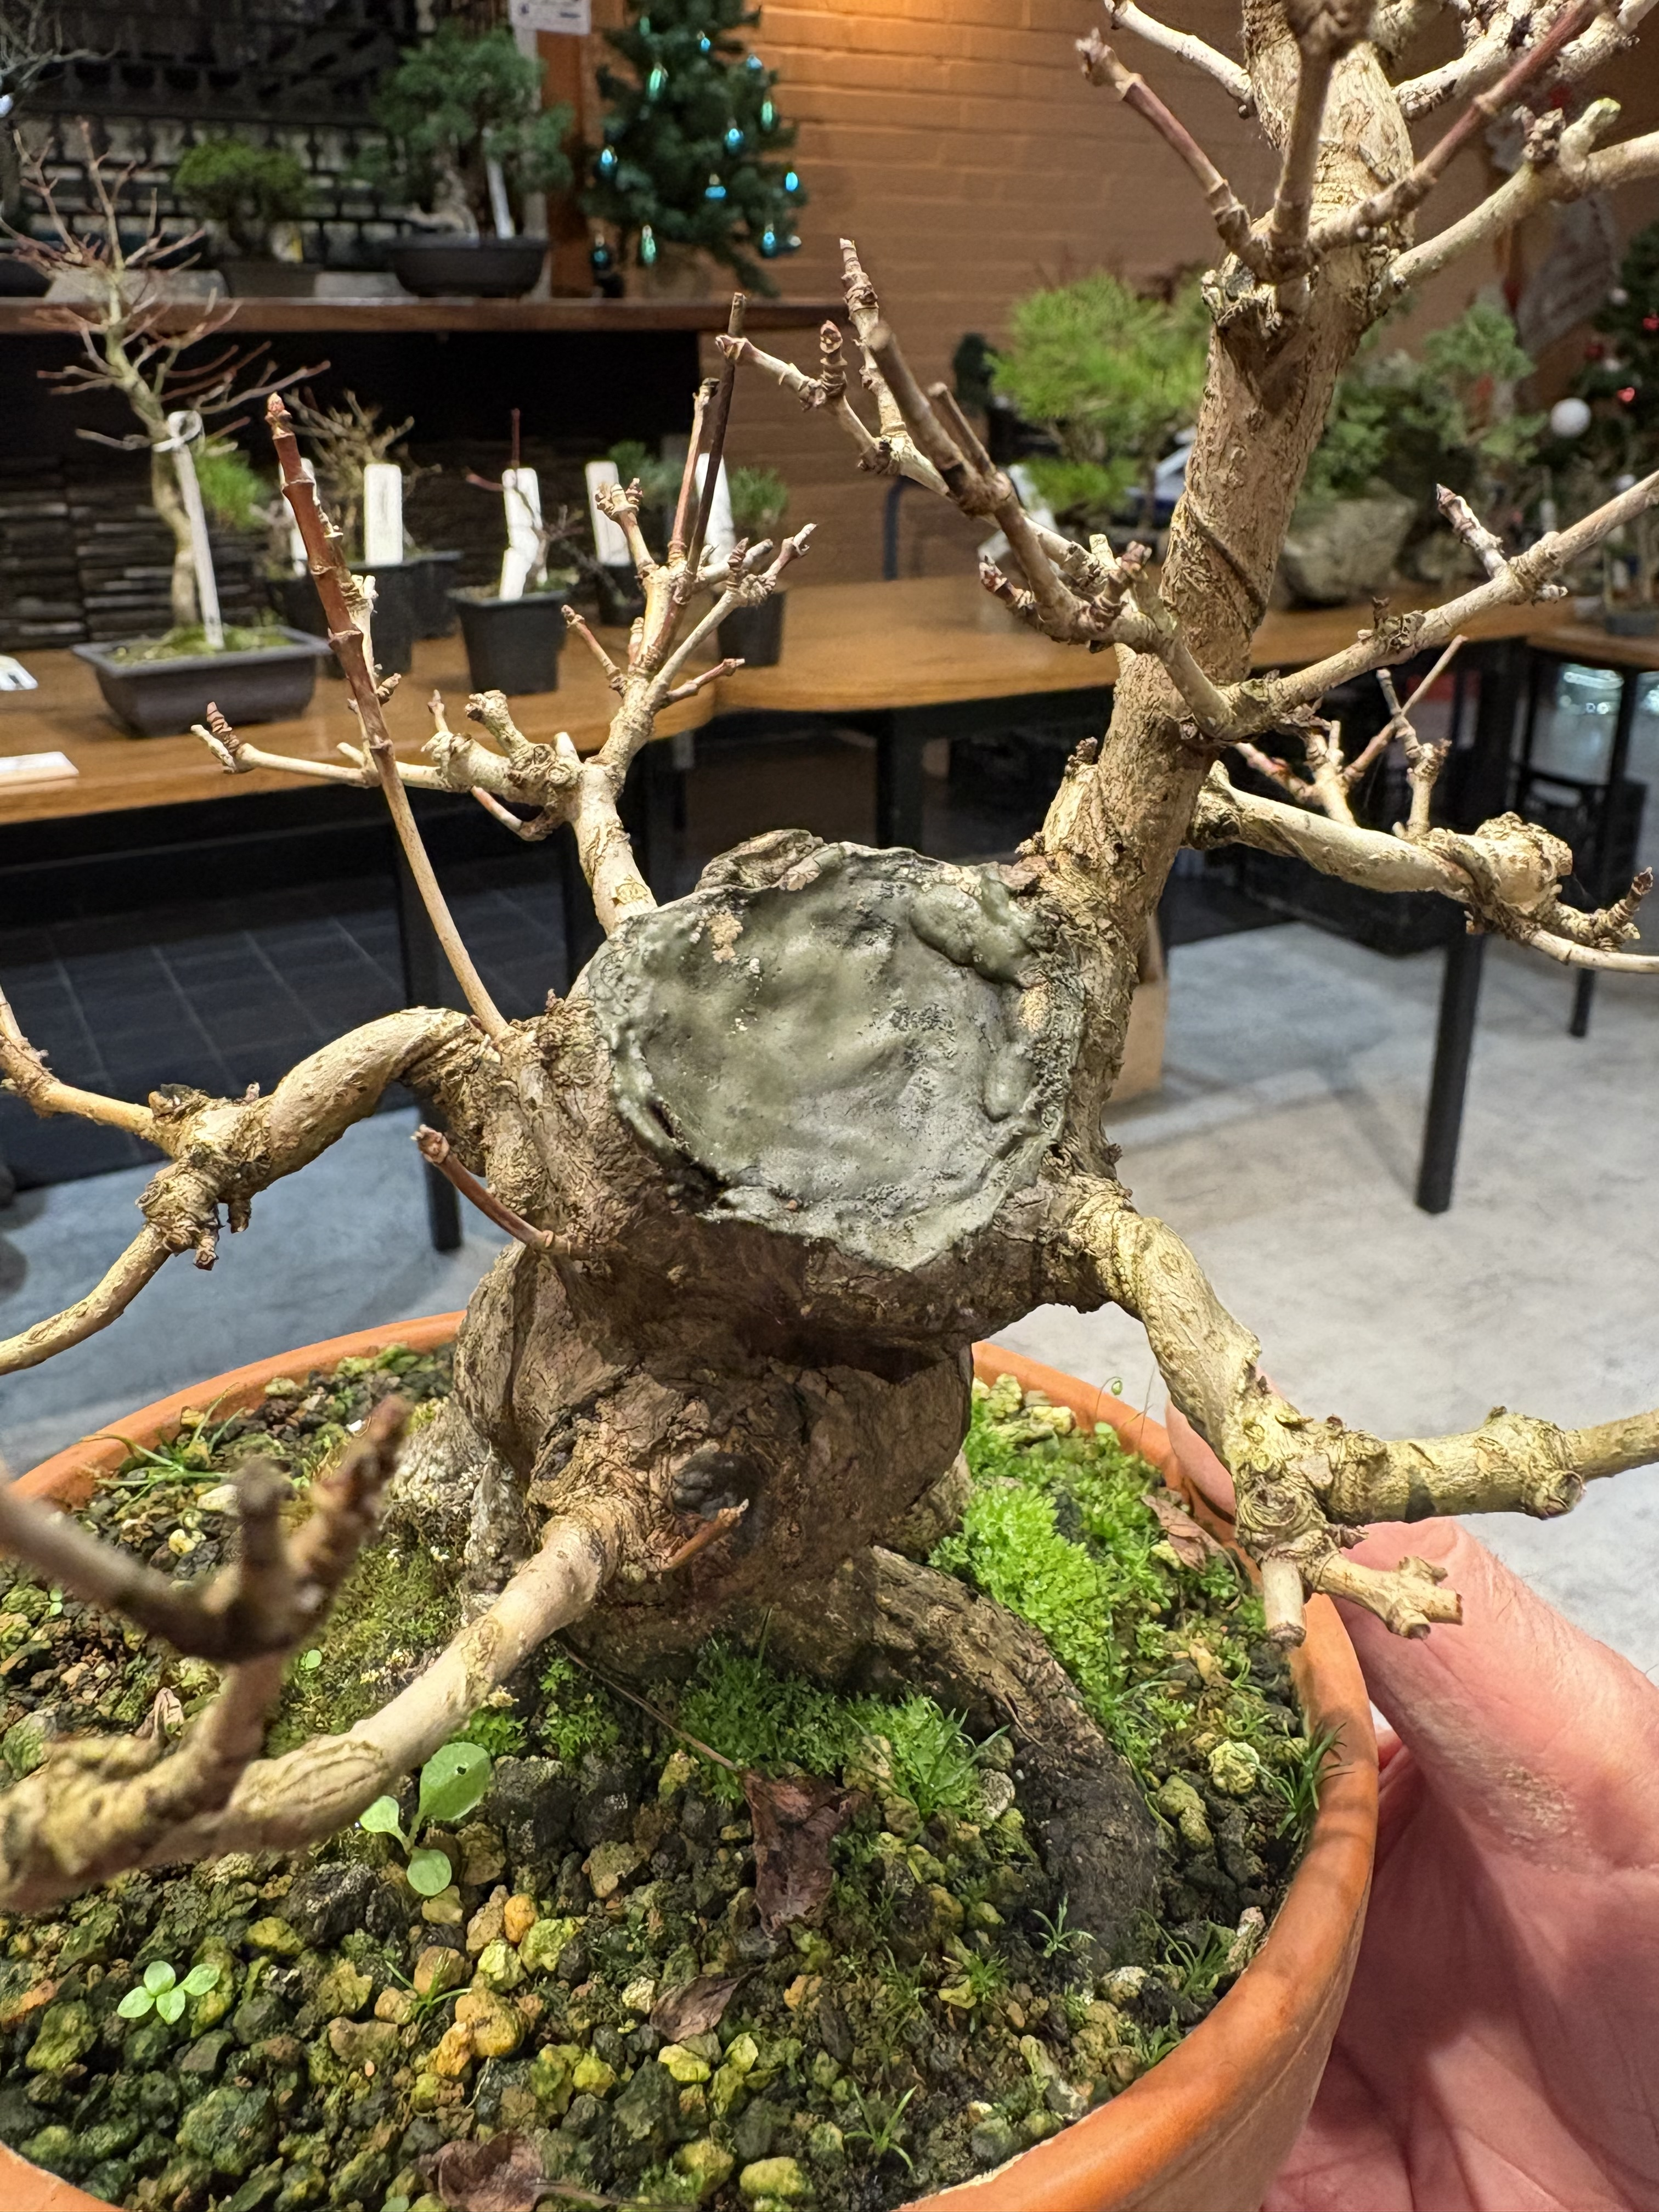
\includegraphics[angle=0,origin=c,width=1.0\textwidth]{2025_11/res/workshop_sacrifice_02.jpg}
\end{minipage}
\end{center}
\centerline{\emph{Grafting and sacrifice branches can help shape the canopy and close large pruning or air-layer cuts.}}
\vfill
\clearpage

\begin{multicols}{2}

\begin{window}[2,l,\includegraphics[width=1.0\columnwidth]{2025_11/res/workshop_sales.jpg},\centerline{\emph{David's wide range of example materials.}}]
\end{window}

\medskip
\topic{Natural Growth and Bonsai Philosophy}
\noindent
A core principle in bonsai cultivation is fostering natural, organic growth rather than creating overly perfect or artificial forms. Imperfections, twists, and asymmetry contribute to character and visual interest. Bonsai should appear as if shaped entirely by nature, with human intervention subtly guiding rather than dominating the tree’s form.  

Historical practices in Japan illustrate this philosophy. Trees maintained by the Imperial Palace before World War II were largely natural bonsai, grown slowly without intensive wiring. Many of these trees survived displacement and naturalization, developing twisted bases and complex branch structures over decades. This naturalistic approach contrasts with modern interpretations that often emphasize precision and symmetry. Appreciating the slow, imperfect development of trees fosters a deeper connection to the art of bonsai and its representation of natural landscapes in miniature.

\medskip
\topic{Feeding, Watering, and Environmental Adaptation}
\noindent
Watering and feeding practices are tailored to a tree’s stage of growth and pot size. Trees in smaller pots are deliberately limited in water and nutrients to control growth and encourage proportionate development. Conversely, trees in larger containers or the ground can receive abundant water and nutrients to stimulate trunk thickening and root expansion.  

Adjusting to environmental changes is crucial after repotting or root reduction. Trees may initially continue vigorous growth, so careful monitoring of irrigation and fertilization ensures survival and gradual acclimatization. Fertilization schedules differ based on species, pot size, and growth phase, with deciduous trees ceasing feeding during dormancy while evergreens may receive dilute nutrient applications. The goal is to maintain healthy, balanced growth that complements the tree’s natural form and environmental conditions.

\medskip
\topic{Advanced Techniques: Layering and Root Exposure}
\noindent
Bonsai enthusiasts employ techniques such as layering and root exposure to enhance visual complexity. Low-hanging branches that touch the ground can form secondary roots, creating naturalistic nebari and supporting semi-cascade or cascade forms. Exposing roots gradually, using tools like tweezers or chopsticks, encourages character without shocking the tree.  

These methods take several years to fully develop. The combination of layered root systems, controlled growth, and selective pruning results in mature-looking bonsai from relatively young material. Patience, observation, and incremental interventions are essential to achieving a tree that balances naturalism with aesthetic appeal.

\medskip
\topic{Practical Nursery Management and Scaling Techniques}
\noindent
Managing a bonsai nursery involves strategic planning to accommodate hundreds or thousands of trees efficiently. Minimal wiring reduces labor while still guiding growth, allowing large collections to be maintained without excessive work. Branches can be manipulated using existing wires, and selective pruning ensures growth follows desired patterns with limited intervention.  

Species selection, potting strategies, and careful observation facilitate predictable outcomes while maintaining tree health. By prioritizing smaller, manageable trees, nurseries optimize space, labor, and material handling, making bonsai cultivation accessible and sustainable over the long term.

\medskip
\topic{Learning from Japan: Trips, Observation, and Cultural Insight}
\noindent
Immersion in Japanese bonsai culture provides invaluable knowledge. Visits to nurseries, gardens, and exhibitions reveal advanced propagation methods, tree management techniques, and design philosophies. Observing naturalistic growth, historical specimens, and layered root structures informs best practices.  

Travel also emphasizes logistical considerations. Japan’s size necessitates careful planning; internal flights or extended train travel are often required to reach key nurseries and gardens. Working with local guides or contacts familiar with language and culture enhances the experience, allowing deeper understanding of techniques, pricing, and tree selection.  

Beyond technical insight, travel highlights the cultural integration of bonsai within broader horticultural practice, including aesthetic preferences, naturalistic design, and historical continuity. Observation, guided participation, and documentation of these experiences are vital for translating traditional practices into personal cultivation.

\medskip
\topic{Shaping Philosophy and Aesthetic Appreciation}
\noindent
The overarching principle of bonsai is to balance human guidance with respect for natural processes. Trees should convey a sense of life and authenticity, with asymmetry, twisted trunks, and irregular branch placement adding depth and character. Overly perfect, symmetrically wired trees can appear artificial, while naturalistic development, supported by minimal intervention, produces enduring beauty.  

Observation over years, rather than instantaneous transformation, ensures trees mature gracefully. The slow accumulation of twists, branch dieback, and root exposure contributes to storytelling within each specimen. Appreciation of these subtle changes aligns with traditional Japanese aesthetics, where wabi-sabi values imperfection and transient beauty.  

Bonsai cultivation is not only about technical skill but also about patience, observation, and respect for nature’s rhythm. Practitioners learn to guide growth thoughtfully, respond to environmental conditions, and embrace the inherent quirks of each tree.  

\medskip
\topic{Conclusion: Integrating Knowledge and Practice}
\noindent
Successful bonsai cultivation requires integration of practical techniques, species knowledge, environmental awareness, and philosophical understanding. Trees respond dynamically to pot size, soil, water, and nutrient availability, while shaping and wiring must harmonize with natural growth tendencies.  

Species-specific strategies, including cutting propagation, layering, and root exposure, allow young trees to develop complex forms over years. Smaller, manageable trees facilitate consistent care and reduce physical strain for practitioners, emphasizing longevity in practice.  

Exposure to Japanese bonsai traditions, coupled with careful observation and patient experimentation, informs both aesthetic and technical development. Ultimately, bonsai is a living art that balances control and natural expression, creating miniature landscapes that reflect patience, skill, and the beauty of imperfection.  
\closearticle

\begin{window}[2,l,\includegraphics[width=1.0\columnwidth]{2025_11/res/workshop_rock.jpg},\centerline{\emph{David’s methods can greatly improve any composition.}}]
\end{window}

\columnbreak

\begin{window}[2,l,\includegraphics[width=1.0\columnwidth]{2025_11/res/workshop_bonsai_01.jpg},]
\end{window}
\vfill

\begin{window}[2,l,\includegraphics[width=1.0\columnwidth]{2025_11/res/workshop_bonsai_02.jpg},]
\end{window}
\vfill

\begin{window}[2,l,\includegraphics[width=1.0\columnwidth]{2025_11/res/workshop_bonsai_03.jpg},\centerline{\emph{A more mature example of David's work.}}]
\end{window}

\clearpage
